\chapter{Theoretical Foundations and State of the Art}
\label{cha:chapter_2}
This chapter establishes the theoretical basis and provides the necessary background required to thoroughly understand the context and scope of \acrlong{dpp} systems. Initially, fundamental concepts and definitions, along with architectural components that characterize \ac{dpp} systems, are outlined in \Cref{sec:dpp_concept_architecture}. Following this, the relevant regulatory frameworks and their specific explicit and implicit requirements for the implementation of \ac{dpp} systems are described in \Cref{sec:regulatory_landscape}. Subsequently, a comprehensive technological analysis is performed, evaluating most relevant existing enabling technologies for \ac{dpp} realization in \Cref{sec:technology_review}. Finally, the chapter concludes by explicitly identifying and discussing existing research gaps, clearly delineating these from the present study, and introducing the research questions that emerge from these gaps (\Cref{sec:research_gaps}).

The theoretical foundations and the assessment of the current state of research presented in this chapter are based on a systematic literature review. The literature review was conducted following a structured research strategy, detailed in \Cref{cha:anhang_A}. The primary sources of information utilized in this literature review are summarized in \Cref{tab:research_resources}.

\begin{table}[htbp]
    \centering
    \caption{Research Resources}
    \begin{tabularx}{\textwidth}{|>{\centering\arraybackslash}X|>{\centering\arraybackslash}X|>{\centering\arraybackslash}X|>{\centering\arraybackslash}X|}
        \hline
        \rowcolor{myDarkBlue}\color{white}\textbf{Library} & \color{white}\textbf{Database} & \color{white}\textbf{Publisher} & \color{white}\textbf{Reference Management} \\
        \hline
        \rowcolor{lightgray!25}OPAC (TUM) & Google Scholar & Springer Nature & Citavi  \\
        \hline
        \rowcolor{myGrey} & Scopus & IEEE & \\
        \hline
        \rowcolor{lightgray!25} & IEEE Xplore & Elsevier & \\
        \hline
        \rowcolor{myGrey} & Connected Papers & ACM & \\
        \hline
        \rowcolor{lightgray!25} & ScienceDirect & MDPI & \\
        \hline
    \end{tabularx}
    \label{tab:research_resources}
\end{table}


\section{Digital Product Passport: Concept and Architecture}
\label{sec:dpp_concept_architecture}

\subsection{Definitions and Core Principles}

As established in the Introduction (\Cref{cha:chapter_1}), the \acrlong{dpp} is a structured digital data representation of a product throughout its lifecycle, facilitating sustainability, traceability, and compliance with environmental standards. The concept has been institutionalized within the \ac{eu} regulatory framework, particularly through the \acrlong{espr}, which mandates its implementation across various product categories. However, beyond its regulatory foundation, the \ac{dpp} embodies a set of core principles and functional attributes that define its role in the circular economy, supply chain transparency, and digitalization of product data. \autocite{EuropeanParliamentandCouncil.2024}

\subsubsection*{\ac{dpp} as a Data Infrastructure}
At its core, the \ac{dpp} serves as an integrated data infrastructure that enables the collection, storage, and exchange of structured product information across the entire value chain \autocite{Jansen.2023}. Unlike traditional product documentation, which is often static and fragmented across multiple stakeholders, the \ac{dpp} ensures a dynamic, real-time flow of product data, thereby enabling:

\begin{itemize}[itemsep=0.5\baselineskip]
    \item \textbf{Regulatory Compliance:} The \ac{dpp} integrates legally required product data, ensuring alignment with sustainability reporting standards, repairability mandates, and material traceability requirements, as outlined in the \acrlong{espr}. \autocite{EuropeanParliamentandCouncil.2024}
    
    \item \textbf{Data Continuity Across the Lifecycle:} The passport consolidates information from raw material extraction to end-of-life recycling, ensuring data persistency across multiple ownership and usage cycles. \autocite{Jansen.2023}
    
    \item \textbf{Multi-Stakeholder Interoperability:} Unlike proprietary tracking systems, \ac{dpp}s function as cross-sectoral, standardized data frameworks designed to facilitate communication between manufacturers, suppliers, regulators, recyclers, and consumers. \autocite{Pietron.2023}
\end{itemize}

Thus, per initial \ac{eu} objectives, the \ac{dpp} is not supposed to be merely a new regulatory compliance mechanism but rather a comprehensive digital tool designed to optimize resource flows, promote sustainable design choices, and support circular business models. \autocite{EuropeanParliamentandCouncil.2024}

\subsubsection*{\ac{dpp} Guiding Principles}
The effectiveness of a \ac{dpp} system is contingent upon several foundational principles, which guide its design, implementation, and long-term viability. These principles have been identified through a synthesis of policy mandates, industry research, and emerging academic discussions.

\begin{enumerate}[itemsep=0.5\baselineskip]
    \item \textbf{Standardization and Interoperability}  
    One of the foremost challenges in \ac{dpp} implementation is the lack of standardization across industries and regulatory domains. The \ac{espr} mandates that \ac{dpp}s adopt harmonized data structures, ensuring that product data remains accessible and interpretable across different platforms and stakeholders. \autocite[1781, Articles 9 and 10]{EuropeanParliamentandCouncil.2024}

    Key aspects of standardization include:
    \vspace{5pt}
    \begin{itemize}
        \item \textbf{Uniform Data Taxonomies:} Establishing common classification systems for product attributes, lifecycle stages, and sustainability parameters. \autocite{HerasSaizarbitoria.2024}
        \item \textbf{Semantic Data Models:} Using semantic frameworks to ensure machine-readable and interpretable datasets, improving automation and \ac{ai}-driven analytics.\autocite{Kebede.2024}
        \item \textbf{Cross-Platform Compatibility:} Ensuring integration with existing \ac{erp} systems, supply chain management tools, and digital twin platforms. \autocite{Pietron.2023}
    \end{itemize}

    \item \textbf{Transparency and Data Accessibility}  
    Transparency is a cornerstone principle of the \ac{dpp}, enabling both consumers and businesses to make informed decisions about product sustainability. The \ac{espr} mandates open access to \ac{dpp} data for regulatory bodies and end-users, fostering accountability across the supply chain. \autocite[1781, Articles 9, 10 and 15]{EuropeanParliamentandCouncil.2024}

    Nevertheless, balancing transparency with data confidentiality remains a challenge, requiring \ac{rbac} mechanisms that determine:
    \vspace{5pt}
    \begin{itemize}
        \item Who can view, modify, or validate product data (e.g., manufacturers, recyclers, regulators).
        \item Which data fields remain publicly accessible versus restricted. \autocite{Ducuing.2023}
    \end{itemize}

    \item \textbf{\acrlong{ce} Enablement and Lifecycle Integration}  
    Unlike static product certifications, the \ac{dpp} is designed to be dynamic, capturing real-time data updates throughout the entire product lifecycle. This feature supports reuse, remanufacturing, repairability assessments, and end-of-life management, aligning with \acrlong{ce} strategies. \autocite{Kuhn.2025}
    
\end{enumerate}

\subsection{Architectural Components and Structures}

As established, the \acrlong{dpp} is not simply a static dataset but a complex, multi-layered system architecture designed to facilitate data exchange, interoperability, and traceability across supply chains. The effectiveness of a \ac{dpp} system is determined by its structural components, data governance models, and technological foundations, all of which must ensure scalability, regulatory compliance, and well-orchestrated stakeholder integration. \autocite{Nowacki.2023}

\subsubsection*{Core Architectural Layers of a \ac{dpp} System}
The Digital Product Passport can be conceptualized as a multi-layered digital infrastructure, comprising three interdependent architectural layers, as illustrated in \Cref{tab:dpp_system_layers}.

Each of these layers is critical for ensuring that the \ac{dpp} remains a functional, interoperable, and scalable system.

\begin{table}[H]
    \centering
    \caption{\ac{dpp} System Layers}
    \begin{tabularx}{\textwidth}{|>{\centering\arraybackslash}X|>{\centering\arraybackslash}X|>{\centering\arraybackslash}X|}
        \hline
        \rowcolor{myDarkBlue}\color{white}\textbf{Layer} & \color{white}\textbf{Functionality} & \color{white}\textbf{Key Components} \\
        \hline
        \rowcolor{lightgray!25}Data Layer & Stores product-related data. & Product registry, lifecycle databases, environmental impact records. \autocite{Wan.2025, EuropeanParliamentandCouncil.2024} \\
        \hline
        \rowcolor{myGrey} Processing \& Governance Layer & Ensures data sovereignty, regulatory compliance, and controlled data exchange between actors. & Standardized \ac{api}s, data interfaces, governance frameworks, access control, cryptographic verification, Digital Twins \autocite{Ajdinovic.2024} \\
        \hline
        \rowcolor{lightgray!25}User \& Application Layer & Interfaces with industry stakeholders, enables the retrieval, visualization, and automated processing of \ac{dpp} data & Web platforms, identifiers, mobile and industrial access points, dashboards, machine-readable \ac{dpp}s \autocite{EuropeanParliamentandCouncil.2024} \\
        \hline
    \end{tabularx}
    \label{tab:dpp_system_layers}
\end{table}

\subsubsection{The Data Layer}
\textit{Structuring Information Across the Product Lifecycle}

The data layer is the foundation of any \ac{dpp} system, ensuring that reliable, standardized product data is stored, structured, and accessible across various lifecycle stages. 

\begin{table}[htbp]
    \centering
    \small
    \caption{Comparison of Supply Chain Types}
    \renewcommand{\arraystretch}{1.2}
    \begin{tabularx}{\linewidth}{
        |>{\centering\arraybackslash}X
        |>{\centering\arraybackslash}X
        |>{\centering\arraybackslash}X
        |>{\centering\arraybackslash}X
        |>{\centering\arraybackslash}X
        |>{\centering\arraybackslash}X|}
        \hline
        \cellcolor{myDarkBlue}\textcolor{white}{\textbf{Supply Chain Type}} & 
        \cellcolor{myDarkBlue}\textcolor{white}{\textbf{Supplier}} & 
        \cellcolor{myDarkBlue}\textcolor{white}{\textbf{Manufacturer}} & 
        \cellcolor{myDarkBlue}\textcolor{white}{\textbf{Service Provider}} & 
        \cellcolor{myDarkBlue}\textcolor{white}{\textbf{Customer}} & 
        \cellcolor{myDarkBlue}\textcolor{white}{\textbf{Recycling}} \\
        \hline
        \cellcolor{myGrey}\textbf{Linear} & 
        Component production & 
        Product manufacturing & 
        Time-based maintenance & 
        Conventional procurement, return \& disposal & 
        Retaining material value (non-reversible) \\
        \hline
        \cellcolor{myGrey}\textbf{Circular} & 
        Component remanufacturing & 
        Value-retention strategies & 
        Condition-based maintenance & 
        Sustainable procurement \& lifecycle extension & 
        Retaining material value (reversible) \\
        \hline
    \end{tabularx}
    \label{tab:supply_chain_comparison}
\end{table}

In \Cref{tab:supply_chain_comparison}, empirical research highlights the fundamental differences in data management between linear and circular supply chains. This comparison serves the purpose of demonstrating the underlying change of information requirements when transitioning towards fully circular supply chains. \autocite{Jensen.2024}

To support the circular model, \ac{dpp} data structure must be designed with a clear schema that defines essential attributes, relationships, and compliance-relevant information, ensuring consistency and usability across different stakeholders and digital systems.

\begin{figure}[ht]
  \centering
  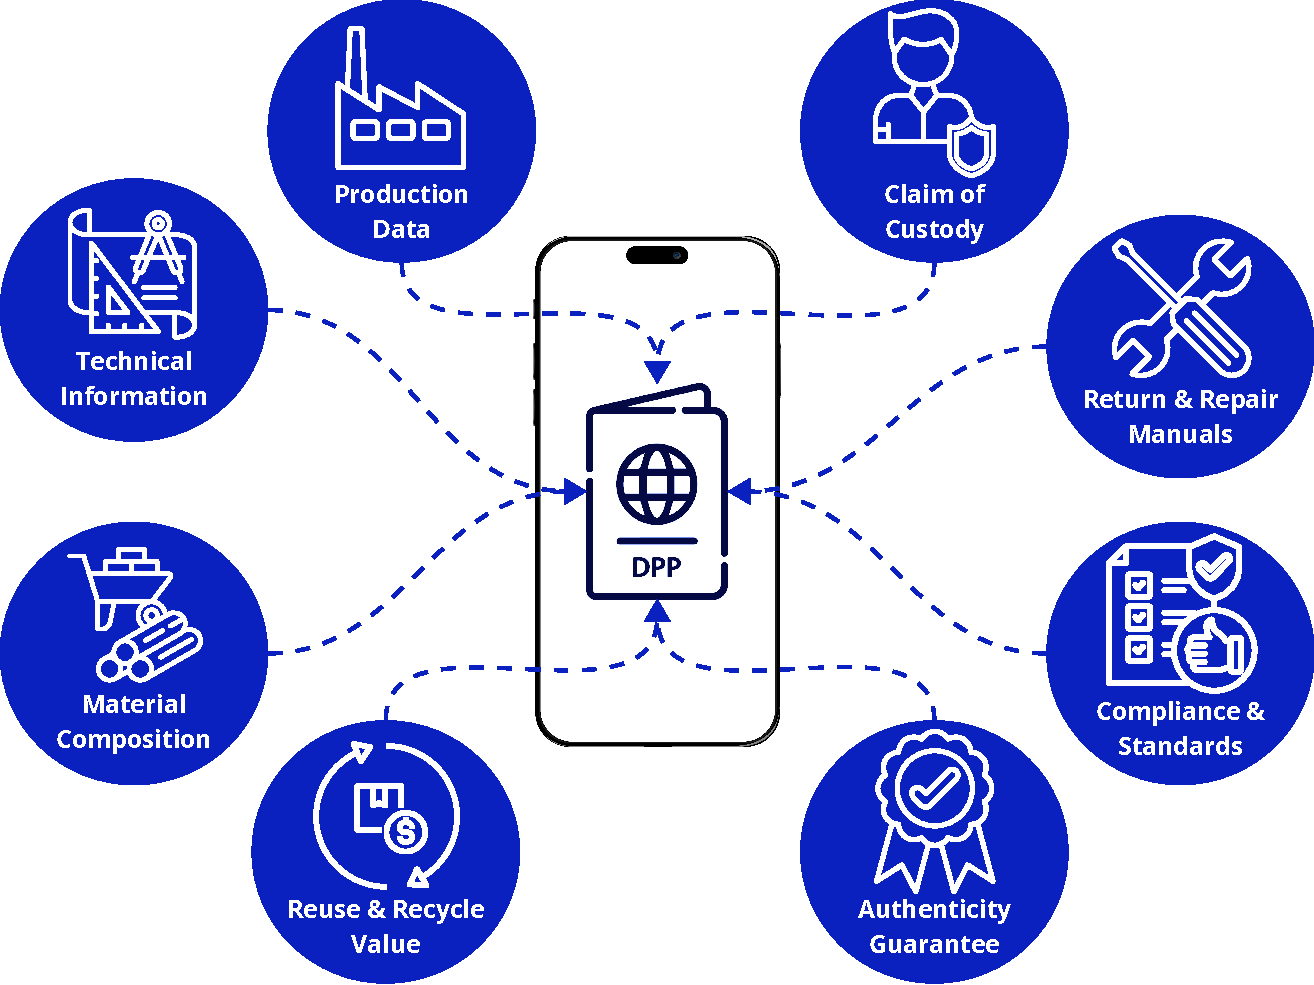
\includegraphics[width=\textwidth]{figures/dpp_data.pdf}
  \caption{%
    \textit{Types of data that should go into a \acrshort{dpp} (Adapted from Circularise, 2024)} 
  }
  \label{fig:dpp_data}
\end{figure}

From an industry perspective, Circularise, a company providing traceability solutions and actively involved in implementing \ac{dpp} solutions, identifies and categorizes key data types relevant for inclusion in a \ac{dpp}, as illustrated in \Cref{fig:dpp_data}. \autocite{Daphne.2024}

Similarly, recent research identifies seven core data clusters that encapsulate the key information required for \ac{dpp} effectiveness across the supply chain. \autocite{Jensen.2023}

\begin{enumerate}[itemsep=0.5\baselineskip]
    \item \textbf{Product Identification Data:}  
    \vspace{5pt}
    \begin{itemize}
        \item Unique product identifier (e.g., serial number, batch codes, EPC, digital link).
        \item Manufacturer and supplier details (company name, production date, batch number, etc.).
        \item Production location and date.
        \item Product category and classification (aligned with \textit{ISO/DIS 59004}).
    \end{itemize}

    \item \textbf{Material and Component Information:}  
    \vspace{5pt}
    \begin{itemize}
        \item \ac{bom} specifying all components and substances.
        \item Material composition, including hazardous substances (aligned with REACH and RoHS).
        \item Percentage of recycled content and traceability of secondary raw materials.
    \end{itemize}

    \item \textbf{Environmental Data:}  
    \vspace{5pt}
    \begin{itemize}
        \item Carbon footprint and Life Cycle Assessment (LCA) metrics.
        \item Water consumption, land use, and toxicity indicators.
        \item Compliance with sustainability reporting frameworks (e.g., PEF, GHG Protocol).
    \end{itemize}

    \item \textbf{Usage and Maintenance Data:}  
    \vspace{5pt}
    \begin{itemize}
        \item Operational history (e.g., running hours, power usage, failure logs).
        \item Maintenance and repair records, including service logs.
        \item Environmental exposure data (e.g., temperature, humidity, chemical exposure).
    \end{itemize}

    \item \textbf{Guidelines and Manuals:}  
    \vspace{5pt}
    \begin{itemize}
        \item Assembly, disassembly, and repair manuals to support extended product lifetimes.
        \item Non-destructive disassembly instructions for material recovery.
        \item Standardized maintenance procedures.
    \end{itemize}

    \item \textbf{Supply Chain and Reverse Logistics Data:}  
    \vspace{5pt}
    \begin{itemize}
        \item Product take-back programs and return channels.
        \item Information on remanufacturing, refurbishing, and reuse potential.
        \item Reverse logistics pathways and waste sorting guidelines.
    \end{itemize}

    \item \textbf{Regulatory Compliance Data:}  
    \vspace{5pt}
    \begin{itemize}
        \item Compliance with \ac{espr} and international \ac{dpp} regulations.
        \item Product safety and environmental certification (e.g., \ac{ce} marking, Ecolabel).
        \item Restricted substance declarations.
    \end{itemize}
\end{enumerate}

According to \textcite{Jensen.2023}, these clusters ensure that \ac{dpp}s are comprehensive, standardized, and functionally adaptable across different product categories and industries.

\subsubsection*{Lifecycle Data Management}
A \ac{dpp} is a dynamic entity, continuously evolving throughout the entire product lifecycle. Unlike traditional static product labels, \ac{dpp}s must be updated at various stages, reflecting changes in ownership, condition, compliance status, and circularity potential. \autocite{Jensen.2023}

\textcite{Jensen.2023} also highlight that different stakeholders require different data updates at specific lifecycle points to support product tracking, maintenance, and sustainability decision-making. This necessitates a structured approach to lifecycle data management, ensuring that each actor contributes relevant information while maintaining data integrity and accessibility.

\Cref{tab:dpp_lifecycle_stages} provides an overview of the different lifecycle stages with the corresponding data updates and responsible stakeholders.

\begin{table}[htbp]
    \centering
    \caption{\ac{dpp} Data Updates Across Lifecycle Stages}
    \resizebox{\textwidth}{!}{
    \begin{tabularx}{\textwidth}{|>{\centering\arraybackslash}X|>{\centering\arraybackslash}X|>{\centering\arraybackslash}X|}
        \hline
        \rowcolor{myDarkBlue}\color{white}\textbf{Lifecycle Stage} & \color{white}\textbf{\ac{dpp} Data Updates} & \color{white}\textbf{Responsible Stakeholders} \\
        \hline
        \rowcolor{lightgray!25}\textbf{Manufacturing \& Initial Registration} & Unique ID assignment, material composition, hazardous substances declaration & Manufacturers, suppliers \\
        \hline
        \rowcolor{myGrey}\textbf{Supply Chain \& Distribution} & Transportation footprint, storage conditions, batch tracking & Logistics providers, ERP systems \\
        \hline
        \rowcolor{lightgray!25}\textbf{Usage \& Maintenance} & Service logs, condition monitoring, repair history updates & Maintenance providers, IoT sensors \\
        \hline
        \rowcolor{myGrey}\textbf{End-of-Life Processing} & Recycling pathways, disassembly guidelines, waste sorting details & Recycling companies, reverse logistics providers \\
        \hline
        \rowcolor{lightgray!25}\textbf{Regulatory Compliance Updates} & New ESG \& sustainability reporting obligations & National \& EU regulatory bodies \\
        \hline
    \end{tabularx}
    }
    \label{tab:dpp_lifecycle_stages}
\end{table}

Manufacturers assign unique product identifiers and document the BOM and material composition, including hazardous substances, recycled content, and sustainability credentials. They also register products in regulatory databases to ensure \ac{espr} compliance, through capturing data on energy efficiency and lifecycle impact assessments. Data integrity at this stage is crucial because errors can negatively affect downstream recyclability and circular economy applications. \autocite{EuropeanParliamentandCouncil.2024, Jensen.2023, Kuhn.2025}

Supply chain actors contribute logistical and transport data by recording shipping conditions (e.g., temperature, humidity, shock absorption), monitoring carbon footprint contributions, and ensuring product authentication during global trade. They also log warehouse conditions, though challenges remain due to interoperability issues between global platforms and \ac{dpp} systems. \autocite{Jensen.2024, Pietron.2023}

Once products reach consumers or businesses, \ac{dpp}s must be updated with maintenance and repair logs, performance data, especially for industrial equipment and consumer electronics, and consumer interaction records for warranty claims and recall management \autocite{Jensen.2024}. In sectors like automotive and industrial machinery, \ac{iot} sensors can provide real-time condition monitoring and predictive maintenance data, although verifying the accuracy of service records remains a challenge \autocite{Pietron.2023}.

At end-of-life, \ac{dpp} data is essential for recycling, remanufacturing, and responsible disposal. This includes documenting which components can be extracted, reused, or recycled, providing details on collection points and manufacturer take-back programs, and ensuring hazardous material handling complies with regulatory requirements. \autocite{Jensen.2024, EuropeanParliamentandCouncil.2024} Notably, \textcite{Jensen.2023} point out that many existing \ac{dpp} models lack comprehensive end-of-life tracking, limiting their \ac{ce} effectiveness.

Beyond core lifecycle stages, \ac{dpp}s must adapt to evolving regulatory frameworks by periodically updating sustainability declarations based on new \ac{esg} mandates, revising hazardous material disclosures as regulations change, and integrating with national product registries to maintain market access. \autocite{Jensen.2023, Pietron.2023, EuropeanParliamentandCouncil.2024}

An emerging paradigm in \ac{dpp} automation is event-driven data aggregation, where product lifecycle data updates dynamically based on real-time events occurring in manufacturing, logistics, and product usage phases. Instead of relying solely on static product records, event-based architectures continuously integrate new process data, so that \ac{dpp} information remains up to date and reflects the actual product status. This approach enhances traceability and  compliance by structuring data according to predefined event models. In manufacturing environments, event-driven \ac{dpp}s allow for automated sustainability tracking. Key metrics such as material sourcing, carbon footprint, and energy consumption are logged and updated in response to real-world events. As research progresses, further integration of these technologies will be essential for ensuring that \ac{dpp}s evolve beyond static product records and into intelligent, self-updating digital assets that promote circular business models, sustainability, and efficiency in industrial processes. \autocite{Ajdinovic.2024, Plociennik.2022}

Despite the benefits of real-time \ac{dpp} updates, several challenges persist in managing lifecycle data effectively. Many \ac{dpp}s are incomplete, particularly in later phases such as recycling and end-of-life tracking, and ensuring accuracy in decentralized update models is problematic given the involvement of multiple stakeholders. Governance ambiguity further complicates matters, as the responsibility for long-term data updates beyond manufacturing is unclear, especially in second-hand markets and recycling facilities, and the credibility of maintenance logs and repair records remains difficult to verify without robust auditing mechanisms \autocite{Ducuing.2023}. Additionally, the absence of standardized data-sharing protocols and the divergence of industry-specific reporting formats impede effective interoperability across manufacturers, recyclers, and regulatory agencies \autocite{Plociennik.2023}.

\subsubsection*{Data Storage Models}
The selection of an appropriate data storage and management architecture directly influences the scalability, security, data integrity, and responsiveness of a \ac{dpp} system. Given the breadth of data categories and lifecycle updates, storage solutions must provide robust data accessibility and integrity for diverse stakeholders, including regulators, industry consortia, manufacturers, suppliers, and consumers. \autocite{Pietron.2023}

The literature identifies three primary data storage models for \ac{dpp} systems - centralized, decentralized, and federated (hybrid) - each with distinct trade-offs in terms of data governance, security, and system architecture.

\subsubsection*{1. Centralized Storage Models}
In the centralized storage method, the data is managed by a single authority, such as a regulatory agency, industry consortium, or private entity. This model facilitates direct regulatory oversight, ensuring that product data remains structured and verifiable within a single system. However, critics highlight concerns regarding data ownership, industry reluctance, and the increased risk of security breaches in a singular repository. \autocite{Pietron.2023}

The key advantages of a centralized \ac{dpp} system include:

\begin{itemize}[itemsep=0.5\baselineskip]
    \item \textbf{Regulatory Oversight and Compliance:} A centralized model ensures strict regulatory alignment, particularly in use cases like centralized \ac{eu} registries for \ac{dpp} references \autocite{EuropeanParliamentandCouncil.2024}. By maintaining direct control over data standardization and compliance monitoring, authorities can reduce administrative complexity for businesses. \autocite{Jansen.2023}
    \item \textbf{Data Consistency and Standardization:} Standardized storage structures enable consistency across industries by ensuring uniform metadata structures and compliance-relevant information storage on a fundamental level. \autocite{Ducuing.2023}
\end{itemize}

However, the model also presents several challenges:

\begin{itemize}[itemsep=0.5\baselineskip]
    \item \textbf{Single Point of Failure:} A centralized database is inherently vulnerable to cyberattacks, system failures, and data corruption. \autocite{Garcia.2024}
    \item \textbf{Scalability Limitations:} As \ac{dpp} adoption expands, a centralized system may experience performance bottlenecks and database overloads. \autocite{Hulea.2024}
    \item \textbf{Restricted Data Ownership:} Manufacturers and businesses may be hesitant to store proprietary data in a government-controlled repository, fearing competitive disadvantages and lack of flexibility in how they manage their digital product data. \autocite{Pietron.2023}
\end{itemize}

\subsubsection*{2. Decentralized Storage Models}
Decentralized storage models conventionally leverage \ac{dlt} and blockchain networks to provide tamper-resistant, transparent, and autonomous data exchange. Unlike centralized models, where data is stored and controlled by a single authority, or federated models that distribute data across multiple stakeholders under a governance framework, decentralized models eliminate central points of control and rely on \ac{p2p} infrastructure. \autocite{Nowacki.2023}

The decentralized approach enhances data integrity, security, and transparency while enabling self-sovereign data management. It is particularly effective in applications where supply chain traceability, regulatory compliance, and secure product lifecycle tracking are critical. \autocite{Hulea.2024}

Decentralized storage models offer multiple advantages for \ac{dpp}s:

\begin{itemize}[itemsep=0.5\baselineskip]
    \item \textbf{Immutable and Tamper-Proof Records:} Product lifecycle data is stored in an immutable ledger using public, private, or hybrid blockchain architectures.Since data is stored on blockchain networks, records are cryptographically secured and cannot be altered retroactively, ensuring the authenticity of product information. \autocite{Nowacki.2023}
    
    \item \textbf{Resilience and Fault Tolerance:} Unlike centralized storage, which presents a single point of failure, decentralized storage ensures data redundancy and self-verification across multiple nodes, making systems highly resistant to attacks. \autocite{Hulea.2024}
    
    \item \textbf{Complete Data Sovereignty:} A decentralized approach ensures that product lifecycle data ownership remains with the original data generators, granting stakeholders full control over data access, integrity, and governance without reliance on a central authority. \autocite{Plociennik.2023}
    
    \item \textbf{Smart Contracts for Automation:} Smart contracts automate data validation and ensure real-time updates while maintaining cryptographic integrity \autocite{Nowacki.2023}. Some regulatory compliance aspects can be enforced through programmable logic embedded in smart contracts \autocite{Plociennik.2023}.
\end{itemize}

Despite their benefits, decentralized storage models present challenges:

\begin{itemize}[itemsep=0.5\baselineskip]
    \item \textbf{Energy Consumption and Scalability:} Public permissionless blockchain networks, particularly those using Proof-of-Work (PoW), have high energy requirements. \autocite{Androulaki.2018}
    
    \item \textbf{Data Privacy and Compliance:} While decentralization enhances transparency, ensuring compliance with data protection laws remains complex, particularly for sensitive product information. \autocite{EuropeanParliamentandCouncil.2016}
    
    \item \textbf{Standardization and Adoption Barriers:} Interoperability across different blockchain frameworks remains a challenge and interoperability between them is not automatically guaranteed. \autocite{Plociennik.2023}
    
    \item \textbf{Smart Contract Security Risks:} Vulnerabilities in smart contract code or execution logic could lead to exploits or data manipulation, requiring rigorous auditing and governance frameworks. \autocite{Hulea.2024, Nowacki.2023}
\end{itemize}

Blockchain-based \ac{dpp}s have gained traction in the battery industry by enabling decentralized reporting and verification of critical lifecycle data, including material sourcing, production processes, and disposal pathways. Similarly, the electronics industry has explored decentralized \ac{dpp} architectures driven by blockchain technology to facilitate compliance with European e-waste management regulations \autocite{Plociennik.2023}. Beyond circular economy considerations, decentralized \ac{dpp} implementations have gained traction in sectors dealing with high-value goods, notably luxury fashion, watches, and pharmaceuticals, where blockchain-based solutions provide effective measures against product counterfeiting and ensure authenticity \autocite{Nowacki.2023}. Despite these promising applications, critical issues such as scalability, energy consumption, and the establishment of effective governance frameworks remain substantial barriers to broader industry-wide adoption.

\subsubsection*{3. Federated Storage Models}
Federated storage models represent a hybrid approach for \ac{dpp} data management, aiming to balance centralized components with decentralized data ownership. Unlike fully centralized models, where a single entity maintains full control, or fully decentralized models, where no central aggregation exists, federated models distribute data storage across multiple stakeholders while adhering to a common governance framework. \autocite{Koppelaar.2023, Plociennik.2022}

This approach provides standardized data interoperability and regulatory compliance without imposing a single point of failure. Federated storage models have been proposed as a scalable and adaptable solution for \ac{dpp} implementation across diverse industries, particularly in contexts where stakeholders seek data sovereignty while ensuring structured and auditable compliance with sustainability regulations. \autocite{Ducuing.2023}

Federated \ac{dpp} models offer several advantages over strictly centralized or decentralized approaches, making them a viable solution for real-world implementations:

\begin{itemize}[itemsep=0.5\baselineskip]
    \item \textbf{Enhanced Data Security and Redundancy:} Since data is stored across multiple independent entities, there is no single point of failure, mitigating risks of cyberattacks, server failures, or systemic corruption. \autocite{Koppelaar.2023}
    \item \textbf{Improved Scalability for Industry Adoption:} Federated models distribute storage and processing loads, allowing the system to scale efficiently as new participants join. \autocite{Redeker.2024}
    \item \textbf{Distributed Data Ownership:} Instead of a single entity controlling all \ac{dpp} data, multiple stakeholders (manufacturers, suppliers, recyclers, and regulators) store and manage different portions of product-related information while also maintaining a unified data system. \autocite{Koppelaar.2023}
    \item \textbf{Cross-Sector Interoperability:} Data sharing and synchronization occur through common metadata frameworks, \ac{api}-based access points, and regulatory-mandated data formats, ensuring harmonized compliance across multiple industries, supply chains, and jurisdictions, making them more adaptable to evolving regulatory landscapes. \autocite{Plociennik.2022, Jansen.2023}
\end{itemize}

Despite their benefits, federated storage models also present key technical, governance, and regulatory challenges:

\begin{itemize}[itemsep=0.5\baselineskip]
    \item \textbf{Complex Governance Coordination:} Unlike centralized models, federated storage requires strong inter-organizational governance mechanisms to ensure data consistency, dispute resolution, and regulatory oversight.\autocite{Alcayaga.2024}
    \item \textbf{Interoperability Barriers Between Proprietary Systems:} Many manufacturers and suppliers operate legacy \ac{it} infrastructures, making real-time synchronization with federated \ac{dpp} repositories a significant technological challenge. \autocite{Jansen.2023}
    \item \textbf{Varying Compliance Enforcement Across Jurisdictions:} Since federated storage allows industry-specific autonomy, there is a risk of inconsistent compliance practices, particularly in cross-border supply chains. \autocite{Ducuing.2023}
    \item \textbf{Higher Initial Implementation Costs:} Federated architectures require investment in interoperability frameworks, multi-level data exchange protocols, and compliance tracking, which can increase the upfront costs for businesses. \autocite{Redeker.2024}
\end{itemize}

Several ongoing initiatives have explored federated storage as a practical solution for \ac{dpp}s. In the automotive industry, the Catena-X initiative has implemented federated data-sharing models specifically aimed at automotive sustainability reporting, aligning \ac{dpp} standards closely with \ac{eu} regulations \autocite{Jousse.2024, Plociennik.2022}. By enabling distributed data control with standardized regulatory oversight, federated \ac{dpp} systems improve scalability, resilience, and industry collaboration. However, governance frameworks, compliance enforcement, and interoperability mechanisms must be carefully developed to ensure widespread adoption and regulatory alignment in global supply chains.

\subsubsection{The Processing and Governance Layer}
\textit{Managing Data Flows and Compliance}

Whereas the Data Layer is where the data is stored and structured, the Processing and
Governance Layer ensures the system's secure and efficient orchestration. This layer is responsible for managing data flows, enforcing access control, and maintaining interoperability across all
product lifecycle stages. Its role is in determining and orchestrating how product information is validated, authenticated, and shared among stakeholders, balancing transparency with data sovereignty needs. \autocite{Ducuing.2023, Jensen.2024}

A robust Processing and Governance Layer must address:

\begin{enumerate}[itemsep=0.5\baselineskip]
    \item \textbf{Data Access and Interoperability} - Mechanisms that determine who can access, modify, and share \ac{dpp} information, ensuring seamless integration across manufacturers, regulators, consumers, and recyclers. \autocite{Ducuing.2023}
    \item \textbf{Security, Verification, and Compliance Mechanisms} - Methods to authenticate and verify \ac{dpp} data, prevent unauthorized modifications, and ensure alignment with regulatory frameworks such as the \ac{espr}. \autocite{EuropeanParliamentandCouncil.2024, Pietron.2023}
\end{enumerate}

The following subsections explore these aspects in depth.

\subsubsection*{Data Access and Interoperability}
The success of a \ac{dpp} system relies not only on technological feasibility but also on its governance structures. Governance in \ac{dpp} ecosystems is inherently complex due to the involvement of multiple stakeholders across the supply chain, each with different roles, responsibilities, and legal obligations. Key challenges include fragmented stakeholder coordination, lack of standardization, and the complexity of integrating legal mandates such as the \ac{espr} and the \ac{gdpr} into scalable digital frameworks \autocite{EuropeanParliamentandCouncil.2016, Pietron.2023}. Manufacturers, regulators, recyclers, and consumers require access to different aspects of the \ac{dpp}, yet existing governance models vary significantly across industries and jurisdictions \autocite{Ducuing.2023}. The lack of a unified governance model has led to fragmented implementations, creating major barriers to interoperability \autocite{Pourjafarian.2023}. Given these challenges, a governance framework must be established that ensures secure data accessibility, robust authentication mechanisms, and automation while fostering industry-wide interoperability \autocite{Jensen.2024}.

A fundamental requirement for effective \ac{dpp} interoperability is ensuring that only authorized entities can access, modify, or validate product data. Two primary mechanisms have emerged as leading solutions: Centralized access control, such as \ac{rbac} and \ac{abac}, and \ac{did}s. 

\ac{rbac} is a widely implemented framework in digital security, where user access is assigned based on predefined roles within an organizational structure, restricting unauthorized modifications or data retrieval. \ac{rbac} ensures compliance in regulated industries by strictly managing permissions across manufacturers, regulators, and recyclers. However, it requires careful role hierarchy design and administrative oversight \autocite{Ferraiolo.1992}. Conversely, \ac{did}-based frameworks introduce a decentralized authentication model, allowing stakeholders to independently verify identities using cryptographic credentials without relying on a central authority \autocite{Garcia.2024}. This approach enables \ac{ssi}, where product owners control authentication credentials, enhancing data sovereignty and reducing dependency on centralized identity providers. \ac{ssi} aligns closely with \ac{gdpr} principles such as data minimization and the right to be forgotten by limiting unnecessary data exposure \autocite{EuropeanParliamentandCouncil.2016, Hulea.2024}. However, widespread adoption requires standardization of cryptographic protocols and harmonization with existing frameworks to avoid legal ambiguities \autocite{Dalipi.2024}.

Beyond access management, one of the end-goals of \ac{dpp} governance is achieving seamless interoperability. Standardized metadata formats and semantic models define how product lifecycle information is structured, classified, and validated to comply with legislative reporting requirements such as the \ac{espr} \autocite{Reif.2024}. These standards ensure that \ac{dpp} data is machine-readable, semantically aligned, and directly compatible with regulatory frameworks.

In parallel, \ac{api}s and standardized data exchange protocols enable real-time interoperability between proprietary systems \autocite{Jansen.2023}. \ac{api}s serve as controlled access points, ensuring that only authorized stakeholders can retrieve, modify, or validate \ac{dpp} data while maintaining secure and verifiable data flows. Governance frameworks regulate \ac{api} authentication, permission structures, and compliance auditing, ensuring that \ac{dpp} data exchanges remain transparent, legally binding, and resistant to unauthorized tampering. Since \ac{dpp} must integrate with diverse digital ecosystems, standardized \ac{api}s facilitate interoperability between \ac{dpp} platforms and existing compliance, supply chain, and sustainability reporting systems. Cloud-based implementations ensure multi-platform accessibility, allowing stakeholders to retrieve data from both public and restricted databases in real time. \autocite{Redeker.2024}

Interoperability frameworks often follow federated governance models, balancing industry-wide standardization with stakeholder autonomy \autocite{DamjanovicBehrendt.2020}. A key mechanism within federated governance is distributed data registries, where industry participants maintain structured records under a unified metadata schema. These registries define data ownership rights, permissioned access levels, and interoperability mandates, ensuring that \ac{dpp} harmonized data can be exchanged securely between manufacturers, regulatory bodies, and third-party compliance auditors.

A notable real-world example is Gaia-X, an \ac{eu}-backed initiative designed to create a federated data infrastructure for European industries \autocite{Reif.2024}. Gaia-X enforces common metadata standards, semantic data models, and \ac{api} compatibility, allowing cross-sector \ac{dpp} data exchange without relying on a single central authority. Similarly, the Catena-X network, focused on the automotive sector, applies federated data-sharing mechanisms for interoperability but does not establish a governance model in itself \autocite{DamjanovicBehrendt.2020}.

Another emerging governance mechanism for interoperability is the establishment of Data Trusts, which function as legal and technical intermediaries for secure, regulated data sharing. A Data Trust defines explicit access, modification, and usage policies, ensuring that stakeholders only retrieve the \ac{dpp} data they are legally entitled to access \autocite{DigitalAutonomyHub.2020}. By implementing audit trails and cryptographic verification, Data Trusts could enhance accountability and trust in multi-stakeholder \ac{dpp} data ecosystems.

Through structured governance frameworks, \ac{dpp} systems can achieve scalable, transparent, and compliant interoperability, leading to minimization of barriers during cross-industry data exchange.

\subsubsection*{Security, Verification, and Compliance Mechanisms}
Another governance issue is regulatory uncertainty and enforcement mechanisms. While
the European Commission has mandated \ac{dpp} implementation, detailed enforcement mechanisms for compliance monitoring remain under development \autocite{Pietron.2023}. The absence of clear penalties for non-compliance raises concerns about inconsistent adoption patterns in the industry. What is more, data sovereignty and security concerns complicate governance further, as businesses remain reluctant to share proprietary product data without well-defined data access and protection frameworks.

One of the primary concerns in \ac{dpp} security is ensuring the authenticity and integrity of product lifecycle data. As \ac{dpp}s serve as authoritative records for compliance tracking, any tampering, unauthorized modification, or fraudulent reporting poses serious risks to the integrity of the whole system. To address these risks, cryptographic verification mechanisms have been widely proposed as a means to establish trust in \ac{dpp} data \autocite{Garcia.2024, Hulea.2024}. Cryptographic hashing ensures that each product record is assigned a unique, tamper-proof identifier, allowing independent verification of data integrity without exposing sensitive details. Blockchain-based audit trails are another prevalent option for providing an immutable history of product modifications to ensure transparency and accountability in reporting \autocite{Dalipi.2024}. 

Given that some \ac{dpp}s may contain personal or business-sensitive data, ensuring compliance with \ac{gdpr} principles such as data minimization, lawful processing, and the right to be forgotten is critical \autocite{EuropeanParliamentandCouncil.2016, Pietron.2023}. To balance transparency with confidentiality, encryption methods have been proposed as a core feature of secure \ac{dpp} architectures \autocite{Hulea.2024}. Zero-Knowledge Proofs offer an additional layer of anonymity by enabling compliance verification without revealing unnecessary data, ensuring adherence to privacy-preserving mandates such as the \ac{gdpr} \autocite{Zyskind.2015}.  Although Zero-Knowledge Proofs have been recognized as a promising privacy-enhancing technology in decentralized identity verification, their application in \ac{dpp} governance remains an area of ongoing research.

When it comes to compliance, one promising technological approach for automating verification is the integration of smart contracts within blockchain-enabled \ac{dpp} architectures. These self-executing protocols provide automated enforcement mechanisms, minimizing administrative overhead. Smart contracts could serve as self-executing regulatory protocols, ensuring that data modifications, transactions, and access permissions adhere to predefined compliance rules. \autocite{Hulea.2024, Nowacki.2023}

Beyond data verification and compliance monitoring, dispute resolution mechanisms are essential for addressing conflicting compliance claims and regulatory disagreements. Given the complexity of multi-stakeholder \ac{dpp} ecosystems, disputes may arise regarding the validity of reported lifecycle data, product certifications, or regulatory attestations. Blockchain-based arbitration frameworks have been proposed as a means of resolving such disputes efficiently, leveraging immutable product records and predefined governance rules to determine regulatory compliance outcomes \autocite{Jensen.2024}. Additionally, structured regulatory attestation networks facilitate cross-border compliance validation, allowing industry regulators to assess \ac{dpp} data through standardized verification protocols \autocite{Pietron.2023}. By incorporating audit trails and verifiable compliance logs, \ac{dpp} systems can reduce reliance on manual legal interventions, streamlining dispute resolution while maintaining legal enforceability.

To ensure widespread industry adoption, \ac{dpp} security and verification frameworks must continuously evolve alongside regulatory mandates. The dynamic nature of compliance requirements necessitates adaptive governance models that can accommodate updates in legislation, emerging data protection norms, and evolving cybersecurity threats \autocite{Ducuing.2023}. By integrating cryptographic verification mechanisms, automated compliance enforcement, and structured dispute resolution frameworks, \ac{dpp} architectures can achieve regulatory resilience and foster stakeholder trust with accurate, transparent and compliant lifecycle data across global supply chains.

\subsubsection{The User and Application Layer}
\textit{Enabling Stakeholder Access}

The final layer in the \ac{dpp} system layered representation is the user-facing Application Layer, which serves as the primary interface between stakeholders and the product passport. This layer ensures that \ac{dpp} data is accessible, understandable, and usable by diverse set of users, including manufacturers, regulators, recyclers, and most importantly end-consumers. Unlike the underlying data storage and processing layers, which focus on persistence, governance, security, and interoperability, the application layer is dedicated to user interaction, identification mechanisms, and machine-readability of \ac{dpp}s. \autocite{EuropeanParliamentandCouncil.2024} These components collectively ensure that \ac{dpp} information is effectively retrieved, visualized, and utilized for decision-making across various lifecycle stages.

Unlike \ac{erp} and \ac{plm} systems, which are typically closed and organization-specific, \ac{dpp}s are designed for standardized, cross-sectoral accessibility and transparency \autocite{Pourjafarian.2023}. The key purpose of the \ac{dpp} user layer lies in providing structured, regulated, and role-specific data access via digital platforms tailored to each stakeholder's needs. This necessitates the development of intuitive user interfaces, robust authentication mechanisms, and adaptable visualization tools \autocite{Plociennik.2022}. 

\subsubsection*{User-Facing Platforms and Interfaces}
User-facing platforms form the core interaction point for all stakeholders engaging with \ac{dpp} data. Unlike traditional industrial software solutions that are optimized for internal use, \ac{dpp} interfaces must be designed for a broad range of users with varying levels of technical expertise and needs. These interfaces include:

\paragraph{Web and Mobile Applications:}
Digital portals allow stakeholders to retrieve, update, and validate \ac{dpp} information. Web-based platforms are commonly employed by regulators, manufacturers, and industry consortia to manage compliance data and perform audits, while mobile applications facilitate real-time access for consumers and field operators via product-scanning functionalities \autocite{ZervasE..2024}. 

\paragraph{Stakeholder-Specific Dashboards:}
Modern \ac{dpp} implementations integrate role-specific dashboards tailored to the requirements of different user groups. A regulatory authority might require dashboards that highlight compliance reports and sustainability metrics, whereas a manufacturer may prioritize lifecycle analytics and traceability data \autocite{Pourjafarian.2023}. A consumer-facing interface, in contrast, needs to prioritize product descriptors, authenticity certificates, sustainability indicators, and repairability guidelines \autocite{Adisorn.2021, Plociennik.2023}.

Given the sensitive nature of certain \ac{dpp} data, access to user-facing platforms is governed by authentication mechanisms often based on the already discussed \ac{rbac} implementations within the previous layer. This simply ensures that only authorized stakeholders can retrieve, modify, or validate specific data elements, essentially safeguarding proprietary non-public information \autocite{Plociennik.2022}.

In a \ac{ce} model, the lifecycle of a product extends beyond the point of sale, necessitating continuous data contributions from consumers to enrich product histories and support reuse, refurbishment, and recycling initiatives. Research highlights the potential of crowdsourced data integration within \ac{dpp}s, where consumers contribute usage patterns, repair logs, and recycling actions, enhancing real-time product lifecycle tracking \autocite{Voulgaridis.2023}. This user-generated data fosters improved decision-making for secondary markets, enabling resale platforms, repair service providers, and recyclers to access verified, consumer-updated product histories \autocite{Koppelaar.2023}. Additionally, the integration of smart connected devices (e.g., \ac{iot}-enabled appliances) facilitates automated updates to \ac{dpp}s, ensuring accurate condition assessments and potential reuse opportunities without requiring active user input. These mechanisms maintain and track valuable lifecycle data post-purchase as an active part of the \ac{ce}’s data ecosystem, thus reinforcing the principles of Extended Producer Responsibility (EPR). 

\subsubsection*{Identifiers and Carriers}
To enable real-world interaction with \ac{dpp} data, physical scannable identifiers are embedded within products, linking them to their corresponding digital records. Among the most widely used carriers are \acrshort{qr} codes, \acrshort{nfc} chips, and \acrshort{rfid} tags, each serving as a means to store unique product identifiers and facilitate reliable access to the corresponding digital records. \autocite{Wan.2025, Ajdinovic.2024}

Each type of identifier presents distinct characteristics in terms of functionality, accessibility, and security. \ac{qr} codes are cost-effective, widely adopted, and accessible using standard smartphone cameras, making them suitable for consumer-facing applications. \ac{rfid} tags, including \ac{rfid} tags, provide extended reading ranges and bulk scanning capabilities, making them preferable for supply chain automation. \ac{nfc} technology, commonly integrated into smartphones, enables secure, short-range communication, offering enhanced protection against counterfeiting and unauthorized modifications. \autocite{ParagonID.n.d., Wan.2025}

A key consideration in the selection of identification carriers is the trade-off between cost, security, and interoperability. While \ac{qr} codes remain the most economical and versatile option, their lack of security features makes them susceptible to duplication. In contrast, \ac{rfid} and \ac{nfc} solutions offer improved resistance to tampering but come at a higher implementation cost. Additionally, the operational requirements of different industries influence the preferred choice of carriers, where retail and consumer goods often favor \ac{qr} codes for transparency, whereas industrial applications may adopt \ac{rfid} for logistics optimization. In this context, RAIN \ac{rfid}, a passive Ultra High Frequency (UHF) technology, offers fast, long-range, and bulk item identification, making it particularly suitable for industrial industrial use \autocite{TheRAINAlliance.n.d.}. \Cref{tab:identifier_comparison} provides an overview of key characteristics, where \textit{+} indicates a positive attribute, \textit{–} a negative one, and \textit{o} denotes a neutral or mixed evaluation. \autocite{ParagonID.n.d.}

\begin{table}[htbp]
    \centering
    \caption{Comparison of Identification Carriers for \ac{dpp} (Adapted from Paragon ID, 2023)}
    \begin{tabularx}{\textwidth}{|X|c|c|c|c|}
        \hline
        \rowcolor{myDarkBlue} \textcolor{white}{\textbf{Feature}} & 
        \textcolor{white}{\textbf{QR Code}} & 
        \textcolor{white}{\textbf{Barcode}} & 
        \textcolor{white}{\textbf{NFC}} & 
        \textcolor{white}{\textbf{RAIN RFID}} \\
        \hline
        \rowcolor{lightgray!25} Accessible with smartphone & + & o & + & - \\
        \hline
        \rowcolor{myGrey} Line of sight required & - & - & + & + \\
        \hline
        \rowcolor{lightgray!25} Longevity & o & o & + & + \\
        \hline
        \rowcolor{myGrey} Price & + & + & - & - \\
        \hline
        \rowcolor{lightgray!25} Bulk reading capability & - & - & o & + \\
        \hline
        \rowcolor{myGrey} Reading range & o & o & o & + \\
        \hline
        \rowcolor{lightgray!25} Protection against copying & - & - & + & + \\
        \hline
    \end{tabularx}
    \label{tab:identifier_comparison}
\end{table}

As industries work towards integrating \ac{dpp}s, the choice of carriers will be adapted per use case and effective combinations can be chosen to tick more boxes than an individual carrier can do. \autocite{ParagonID.n.d.}

\subsubsection*{Machine-Readable and Automated DPPs}
Beyond human-readable interfaces, \ac{dpp} architectures must support machine-readable formats to enable automated data processing, integration with \ac{ai} systems, or compliance verification. The structuring of \ac{dpp} data into semantic ontologies and standardized data formats (e.g., JSON-LD, XML, OPC UA) ensures that machines can interpret and exchange information seamlessly. \autocite{Kebede.2024, Jansen.2025}

While all data carriers, including \ac{qr} codes, \ac{nfc}, and \ac{rfid}, are inherently machine-readable, their usability varies across different industrial and logistical settings. For instance, RAIN \ac{rfid} technology is particularly advantageous for automated warehouse operations, as it supports bulk scanning without requiring line-of-sight access, unlike traditional barcodes or \ac{qr} codes. These attributes make certain identifier technologies more suited for high-volume industrial applications, while others, such as \ac{qr} codes, remain ideal for consumer-level accessibility. \autocite{ParagonID.n.d.}

The Application Layer provides user-centric interfaces and machine-readable structures, facilitating direct interaction with \ac{dpp} data. Its primary purpose is to enhance data accessibility and transparency through standardized identifiers, intuitive user interfaces, and structured, interoperable data formats. By enabling both human-driven interaction and automated data processing, this layer directly supports the objectives of the \acrlong{ce}. With evolving regulatory requirements, the continued standardization and refinement of \ac{dpp} interfaces will become increasingly critical to achieving mass adoption across different stakeholder groups.

\subsection{Architecture Overview}

The system architecture overviews the overall \ac{dpp} system and integrates the previously discussed layers, clearly defining the interplay among technological components, stakeholders, and data management processes. 

This section consolidates key architectural insights from leading initiatives, including \textit{ZVEI’s Architecture Proposal for a \ac{dpp}-System}, \textit{CIRPASS’s DPP System Architecture}, \textit{GS1 in Europe’s Proposed Architecture and Principles for Digital Product Passports} and \textit{European Commission’s DIGIT Webinar on \ac{dpp} Data Storage and Management}, to provide a high-level overview of how \ac{dpp} systems have already been conceptualized and structured.

A fundamental challenge in \ac{dpp} architecture design is the effective alignment of storage models with overarching data governance frameworks. Storage alone does not determine how \ac{dpp} data is managed, accessed, and maintained over time; rather, governance mechanisms define the rules for data interoperability, lifecycle management, and compliance enforcement. European Commission’s Directorate-General for Informatics (DIGIT) webinar on \ac{dpp} Storage and Data Management highlights key distinctions between storage architectures and data governance responsibilities, emphasizing the need for a well-balanced and clearly defined system design. \autocite{Frade.2023}

As it has already been discussed, a \ac{dpp} system may rely on centralized, federated, or decentralized storage models, each carrying distinct governance implications. \Cref{tab:dpp_storage_data_management_DIGIT} illustrates the alignment and coordination between data storage solutions and data management practices, as identified by the European Commission. Even though the table has been expanded to showcase all of the possible combinations of data hosting and governance models for the sake of comprehensiveness, not all options are economically, legally or even technically feasible. \autocite{Frade.2023}

The configurations presented in \Cref{tab:dpp_storage_data_management_DIGIT} are color-coded according to their alignment with the preferences identified by the European Commission. Specifically, cells highlighted in red represent configurations that were not even considered due to either obscurity or misalignment of the architecture with the ideology behind \ac{dpp}. Cells marked in pink indicate the unsuitable or explicitly discouraged configurations, which do not align well with the ideology behind the \ac{dpp} concept. Lastly, cells indicated in yellow denote preferred and actively considered configurations, clearly aligning with the European Commission’s recommended data governance principles. \autocite{Frade.2023}

\begin{table}[htbp]
    \centering
    \caption{European Commission's Considerations for Storage and Governance (Adapted from DIGIT Webinar, 2023)}
    \renewcommand{\arraystretch}{1.5}
    \begin{tabularx}{\linewidth}{
        |>{\centering\arraybackslash}X
        |>{\centering\arraybackslash}X
        |>{\centering\arraybackslash}X
        |>{\centering\arraybackslash}X|}
        \hline
        \cellcolor{myDarkBlue}\textcolor{white}{\textbf{Data Storage vs. \ac{dpp} Data Management}} &
        \cellcolor{myGrey}\textbf{Centralized Hosting} &
        \cellcolor{myGrey}\textbf{Federated Hosting} &
        \cellcolor{myGrey}\textbf{Decentralized Hosting} \\
        \hline
        \cellcolor{myGrey}\textbf{Centralized Service} & 
        \cellcolor{Salmon}All \ac{dpp} data stored and managed in a central repository. & 
        \cellcolor{Mahogany}Central authority coordinates federated data. & 
        \cellcolor{Mahogany}Centralized authority coordinates decentralized data pieces. \\
        \hline
        \cellcolor{myGrey}\textbf{Federated Services / Based on Service Providers} & 
        \cellcolor{Mahogany}National authorities access and manage data in a central repository. & 
        \cellcolor{Salmon}National authorities provide \ac{dpp} Service. & 
        \cellcolor{Goldenrod}\textbf{OPTION A:} Independent service providers with local data control, requiring registration in federated DPPaaS systems. \\
        \hline
        \cellcolor{myGrey}\textbf{Decentralized Services / Self-Sovereign} & 
        \cellcolor{Mahogany}Economic operators maintain data in a central structure. & 
        \cellcolor{Mahogany}Economic operators control and distribute data across federated services. & 
        \cellcolor{Goldenrod}\textbf{OPTION B:} Economic operators fully self-manage and self-host their \ac{dpp}s. \\
        \hline
    \end{tabularx}
    \label{tab:dpp_storage_data_management_DIGIT}
\end{table}

The European Commission’s stance, as outlined by \textcite{Frade.2023}, indicates a strong preference for hybrid federated architectures, recognizing the importance of structured governance while maintaining data sovereignty for industry stakeholders. Both Option A (Federated DPPaaS) and Option B (Full Decentralization) are considered viable. The key difference lies in governance structure: Option A allows for both complete self-autonomy of economic operators and the use of accredited third-party service providers (entities offering accredited \ac{dpp} solutions), through whom the participants register with federated DPPaaS (Digital Product Passport as a Service) providers to ensure validation and redundancy. Option B assumes complete decentralization without mandatory reliance on third-party providers. Option A, however, appears to be the more versatile choice, effectively combining economic operators' data sovereignty needs with regulators' requirements for federated oversight and interoperability.

\subsubsection*{ZVEI's \ac{dpp} 4.0 Architecture Proposal}
The ZVEI (German Electrical and Electronic Manufacturers' Association) has proposed a robust architecture for the \acrlong{dpp} system, termed \ac{dpp} 4.0. This architecture provides a structured framework that defines the key elements and systems involved in a fully operational \ac{dpp} ecosystem. The architecture distinguishes between different stakeholders and their interactions with different systems, as illustrated in \Cref{fig:dpp_system_overview}. \autocite{Garrels.2023}

\begin{itemize}[itemsep=0.5\baselineskip]
    \item \textbf{Actors:} The primary stakeholders who generate, manage, or consume \ac{dpp} data within the system. These entities are directly responsible for creating and updating product-related records.
    
    \item \textbf{External Actors:} The entities who interact with the \ac{dpp} system but do not directly generate or own the product data. These actors typically have read-only or validation privileges, as defined in by the governance framework. Their role is crucial in regulatory compliance, auditing, and data validation.
    
    \item \textbf{Systems:} These are the core technological components that store, process, and provide access to \ac{dpp} data, the so-called backbone of the \ac{dpp} infrastructure.
    
    \item \textbf{External Systems:} These are external components that facilitate interoperability between the \ac{dpp} framework and regulatory or industry-specific platforms.
\end{itemize}

This breakdown outlines key actors, systems, and external entities within the ZVEI \ac{dpp} 4.0 architecture, demonstrating how best research practices, European regulatory goals, industry standards, and practical considerations can be integrated. It bridges conceptual design and system planning, offering a scalable, standardized, and compliance-oriented \ac{dpp} ecosystem aligned with \ac{eu} directives. \autocite{Garrels.2023}

\begin{figure}[ht]
    \centering
    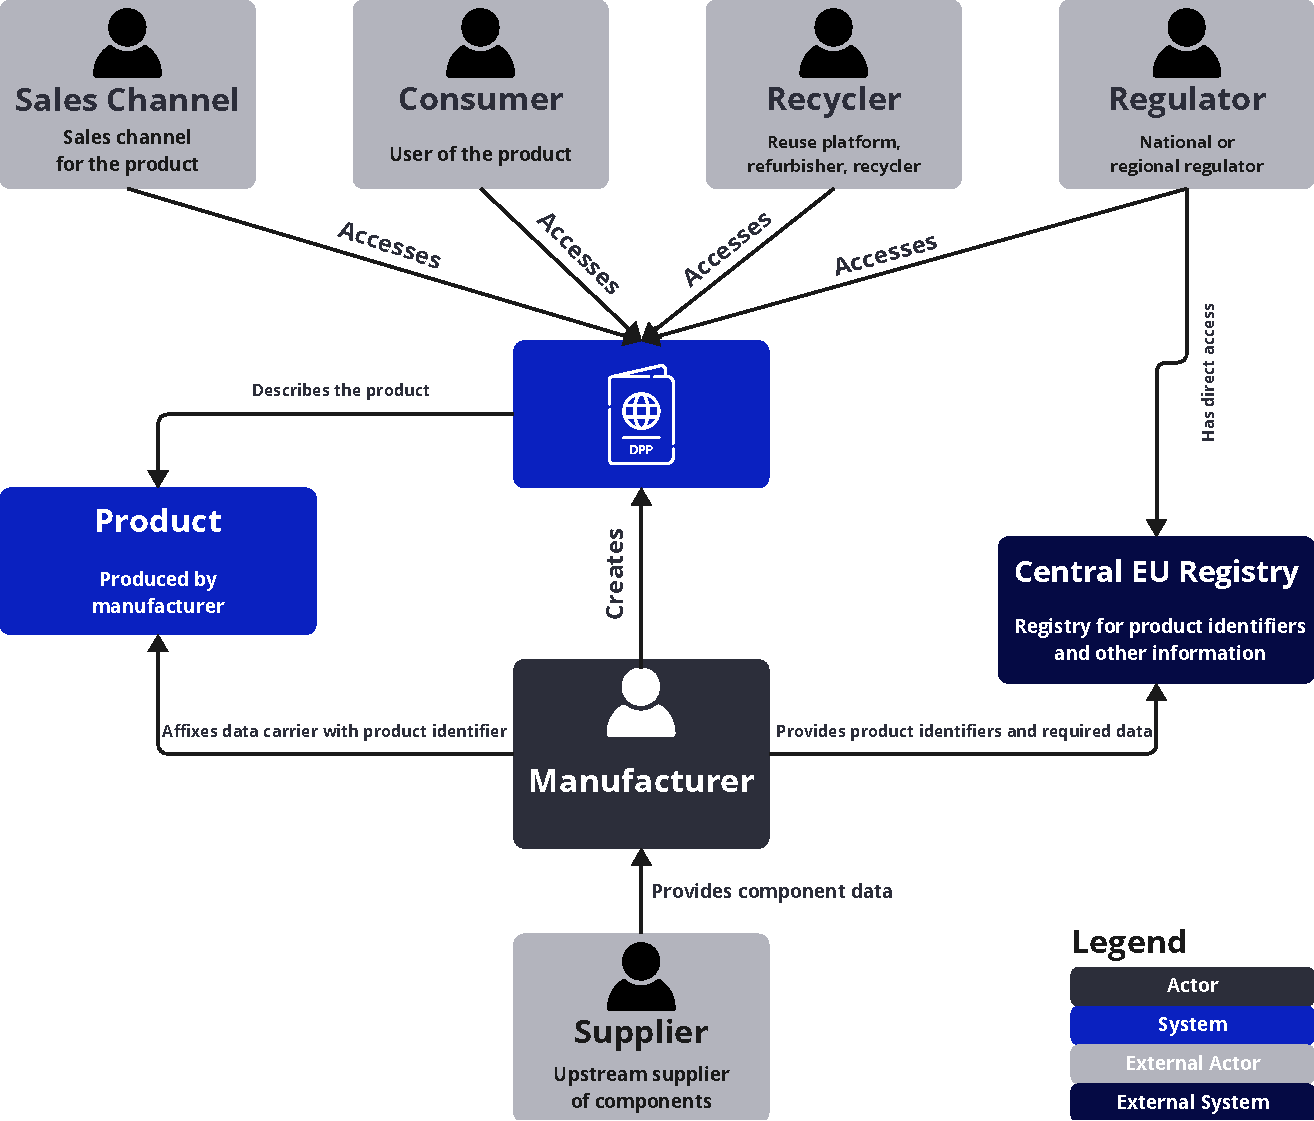
\includegraphics[width=\textwidth]{figures/dpp_system.pdf}
    \caption{Overview of the ZVEI \ac{dpp} 4.0 System and Its Actors (Adapted from ZVEI, 2023)}
    \label{fig:dpp_system_overview}
\end{figure}

Goals of the \ac{dpp} 4.0 System include:

\begin{itemize}[itemsep=0.5\baselineskip]
    \item \textbf{Data Sovereignty} is achieved by advocating for decentralized \ac{dpp} repositories offering HTTP-REST interfaces (\ac{api}s) for controlled access. This approach allows easy integration into existing \ac{it} infrastructures, promoting data sovereignty and reducing reliance on central authorities.
    \item \textbf{Interoperability} is accomplished through the use of standardized data formats, such as OPC UA, JSON-LD, and IEC-based identification schemes, ensuring that different platforms and stakeholders can retrieve \ac{dpp} data without compatibility issues. Additionally, \ac{api} gateways and resolvers ensure that product identifiers remain universally accessible.
    \item \textbf{Low Entry Barriers} is supported by an open and modular system design, where companies can choose from various implementation models, including cloud-based, federated, or fully decentralized repositories. Moreover, the architecture prioritizes widely adopted technologies for accessibility, ensuring that stakeholders can interact with \ac{dpp} data without requiring specialized hardware or proprietary solutions.
\end{itemize}

A core function of the \ac{dpp} 4.0 architecture is supporting structured and secure data access for various stakeholders. The architecture establishes a versatile data flow mechanism ensuring that \ac{dpp} data retrieval is efficient, verifiable, and adaptable to different use cases. The structured interaction process between users, manufacturers, and repositories is illustrated in \Cref{fig:dpp_access_flow}. \autocite{Garrels.2023}

\begin{figure}[htbp]
    \vspace{-10pt}
    \centering
    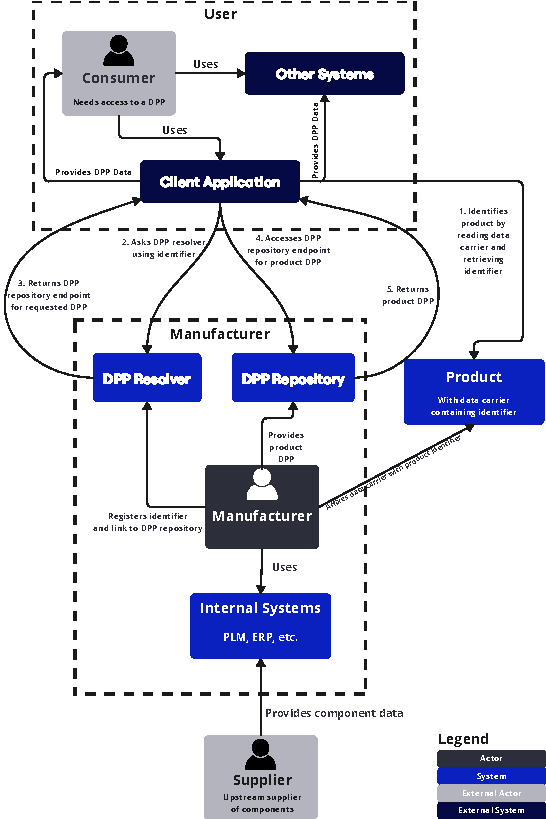
\includegraphics[width=\textwidth]{figures/dpp_access_flow.pdf}
    \caption{Data Flow for \ac{dpp} Access in the Ecosystem (Adapted from ZVEI, 2023)}
    \label{fig:dpp_access_flow}
\end{figure}

The key steps in this data exchange process are as follows:

\begin{enumerate}[itemsep=0.5\baselineskip]
    \item \textbf{Identification of the Product:} The process begins when a user (e.g., consumer, regulator, recycler) attempts to access the \ac{dpp} of a product. The user retrieves the unique product identifier by scanning a physical data carrier (e.g., \ac{qr} code, \ac{nfc} tag, \ac{rfid}).
    \item \textbf{Client Application Requests the Resolver:} The user interacts with a client application that requests the \ac{dpp} resolver. The resolver serves as a lookup service that determines the corresponding repository where the requested \ac{dpp} is stored.
    \item \textbf{Resolver Returns Repository Endpoint:} The resolver responds by providing the repository location that holds the requested \ac{dpp}. This mechanism ensures that decentralized repositories remain accessible and discoverable.
    \item \textbf{Repository Access and Data Retrieval:} The client application then accesses the designated \ac{dpp} repository endpoint. The repository verifies authentication and returns the product’s digital passport data.
    \item \textbf{\ac{dpp} Data Presentation:} The retrieved \ac{dpp} is presented to the user via a structured interface, ensuring that relevant data is accessible in a user-friendly format while maintaining compliance with governance frameworks.
\end{enumerate}

The \ac{dpp} 4.0 data flow model (\cref{fig:dpp_access_flow}) separates the resolver and repository, ensuring manufacturers control storage while global resolution services maintain accessibility. Robust \acrlong{rbac} and authentication ensure that only authorized entities can access or modify records, and the resolver architecture prevents data duplication, always delivering the most accurate product information. By clearly defining resolution, storage, and access control, the ZVEI \ac{dpp} 4.0 proposal offers a scalable, federated model aligned with the European Commission’s vision for digital product passports, leveraging standardized identification, modular information modeling, and decentralized data management to achieve practical data sovereignty, interoperability, and scalability. \autocite{Garrels.2023}

\subsubsection*{CIRPASS \ac{dpp} System Architecture}
Next to the structured and modular approach defined by ZVEI’s \ac{dpp} 4.0 architecture, the CIRPASS initiative provides yet another expanded perspective on \ac{dpp} system design. While ZVEI emphasizes the technical modularity of \ac{dpp} repositories and resolution frameworks, CIRPASS extends this model by explicitly defining how governance, compliance, and data validation mechanisms interact within the system architecture. By incorporating public authorities, autonomous validation, and structured compliance monitoring, CIRPASS ensures that the \ac{dpp} ecosystem is not only technically scalable but also legally enforceable. \autocite{Wenning.2024}

A defining aspect of the CIRPASS architecture is its explicit delineation of system components and stakeholder roles. The model categorizes system actors into economic operators, regulatory bodies, and service providers, each interacting with the \ac{dpp} system at different levels of responsibility. Unlike other models that primarily focus on data exchange between manufacturers and end-users, CIRPASS introduces dedicated compliance checkpoints, explicitly highlighting how market surveillance authorities, customs, and policymakers have structured access to product lifecycle data. This enhances regulatory oversight while maintaining data sovereignty for economic operators managing their own \ac{dpp} instances. While ZVEI defines a decentralized resolver approach, CIRPASS introduces a tiered resolution mechanism, where a centralized \ac{eu} registry plays a more critical role and empowers product data lookup across distributed systems, resulting in an effective and highly-interoperable federated system. \autocite{Wenning.2024, Garrels.2023}

\begin{figure}[htbp]
    \centering
    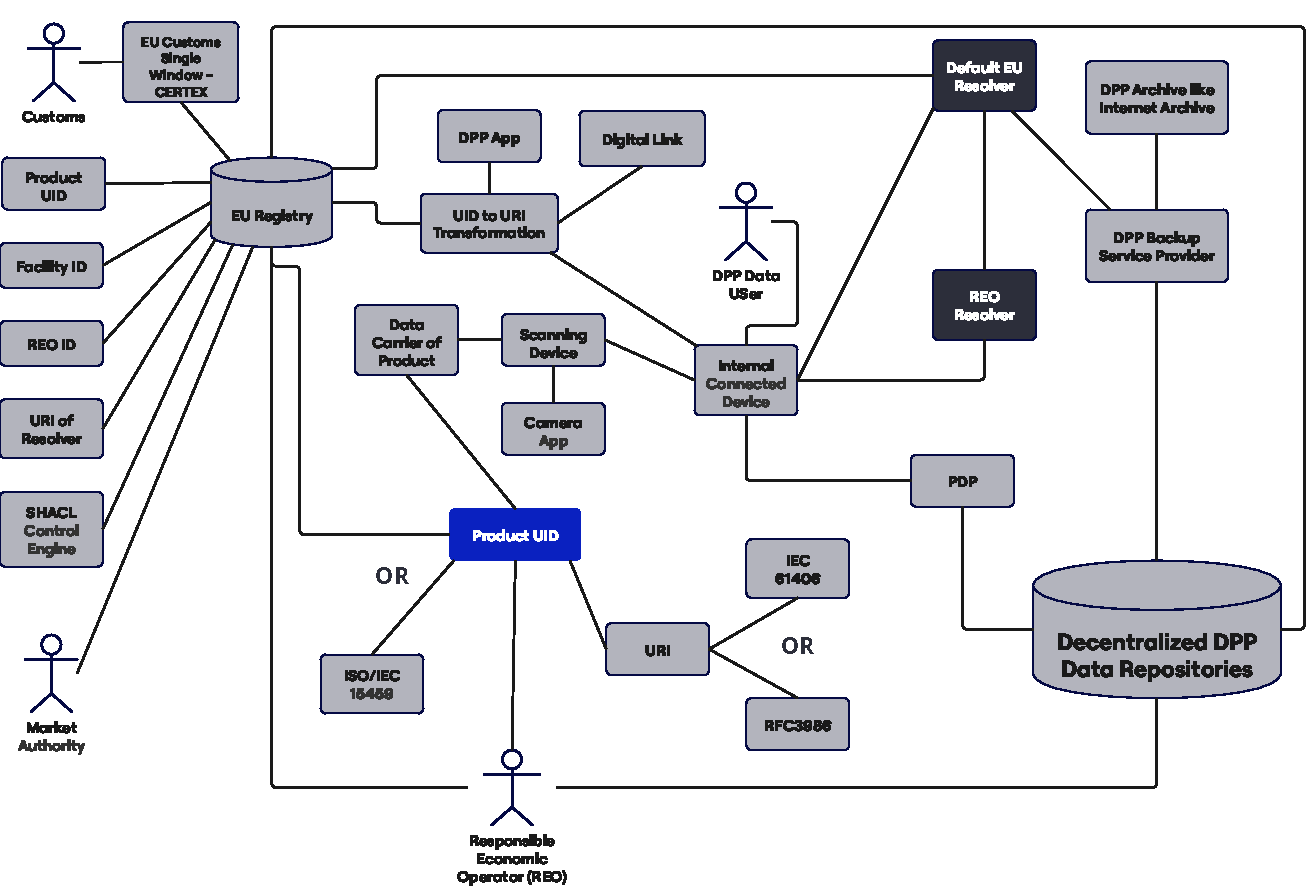
\includegraphics[width=\textwidth]{figures/dpp_cirpass_architecture.pdf}
    \caption{CIRPASS DPP System Architecture Overview (Adapted from CIRPASS, 2024)}
    \label{fig:dpp_cirpass_architecture}
\end{figure}

CIRPASS introduces structured compliance enforcement processes and \ac{eu}-wide governance layers. Each \ac{dpp} instance can undergo validation by accredited bodies before being made accessible to external stakeholders. This ensures that product lifecycle data is not only structured and accessible but also meets predefined compliance requirements before entering the resolution system. Additionally, CIRPASS incorporates policy enforcement layers, ensuring that data retrieval requests adhere to predefined access rules based on the requesting entity’s authorization level. The overall system architecture and the interaction between different system components and stakeholders in the CIRPASS architecture is showcased in \Cref{fig:dpp_cirpass_architecture}. \autocite{Wenning.2024}

The key steps in the CIRPASS data flow are outlined below:

\begin{enumerate}[itemsep=0.5\baselineskip]
    \item \textbf{Product Identification and Query Initiation:} A stakeholder (e.g., consumer, regulator, recycler) retrieves the unique product identifier by scanning a physical data carrier. This triggers a \ac{dpp} resolution request, which is routed to the structured query system.
    
    \item \textbf{Registry and Resolver Mechanisms:} CIRPASS's multi-tiered resolution process has the following components:
    
    \begin{itemize}
        \item EU Registry: Maintains authoritative records linking product UIDs (Product UID, Facility ID, REO ID) to their associated \ac{dpp} repositories.
        \item Resolver Layer: The Default \ac{eu} Resolver and Responsible Economic Operator (REO) Resolver determine the correct repository location for the requested product.
    \end{itemize}
    
    \item \textbf{Compliance Validation and Policy Enforcement:} Before granting access, CIRPASS incorporates a structured compliance checkpoint using a Policy Decision Point (PDP). This mechanism ensures that only authorized and verified \ac{dpp} records are retrieved, preventing data tampering or access by non-compliant actors.

    \item \textbf{\ac{dpp} Retrieval and Access Governance:} After successful validation, the \ac{dpp} repository serves structured product lifecycle data to the requesting entity. CIRPASS ensures compliance and interoperability with semantic standardization by supporting multiple data models (e.g., ISO/IEC 15459, IEC 61406, RFC3986) for interoperability across industries and for specific user needs.
    
    \item \textbf{Backup, Archiving, and Redundancy Measures:} To maintain data resilience, CIRPASS integrates:
    \begin{itemize}
        \item \ac{dpp} Backup Service Providers who provide long-term storage of \ac{dpp} records, preventing data loss.
        \item \ac{dpp} Archiving to maintain historical product lifecycle data as historical snapshots for auditability.
    \end{itemize}
\end{enumerate}

This section has provided a comprehensive overview of \ac{dpp} system architectures, emphasizing how effectively structured data flows, clearly defined governance frameworks, and robust interoperability mechanisms form the foundation for scalable and compliant implementations. By examining leading industry proposals such as ZVEI’s \ac{dpp} 4.0 and CIRPASS's architectural approach, it becomes clear that the successful deployment of \ac{dpp} ecosystems relies on thoughtfully balancing decentralized data sovereignty, federated governance, and semantic compliance. These considerations underline the importance of coherent interaction across data, governance, and application layers, establishing a solid foundation for real-world implementation.

\section{Regulatory Landscape and DPP Requirements}
\label{sec:regulatory_landscape}

\subsection{Introduction to Regulatory Evolution}

The regulatory landscape surrounding \acrlong{dpp}s has evolved significantly over the past several years. Initially, global sustainability initiatives focused on voluntary environmental declarations and supply chain transparency. However, the growing need for product traceability, resource efficiency, and circular economy enforcement led to the structured regulatory frameworks we see today. This section outlines key milestones in the legislative journey toward the establishment of \ac{dpp}s, focusing on the \acrlong{eu}'s leadership in this domain.

The foundation of product sustainability regulations was laid by early directives and voluntary frameworks promoting environmental responsibility and resource efficiency. Key regulatory developments include:

\begin{enumerate}[itemsep=0.5\baselineskip]
    \item \textbf{Registration, Evaluation, Authorisation, and Restriction of Chemicals (REACH) (EC No 1907/2006)} established material transparency requirements that indirectly influenced digital documentation needs in supply chains. \autocite{EuropeanParliamentandCouncil.2006}
    
    \item \textbf{The Waste Framework Directive (2008/98/EC)} established principles for waste prevention, reuse, recycling, and recovery. While not explicitly mandating digital tracking, it laid the groundwork for extended producer responsibility (EPR) schemes. \autocite{EuropeanParliamentandCouncil.2008}
    
    \item \textbf{The Ecodesign Directive (2009/125/EC)} introduced sustainability requirements for energy-related products, promoting life-cycle thinking and efficiency in design. \autocite{EuropeanParliamentandCouncil.2009}
\end{enumerate}

With the rise of digitalization and supply chain complexity, regulators began incorporating digital tools to enhance transparency. The following milestones marked the transition from voluntary sustainability measures to structured regulatory mandates:

\begin{enumerate}[itemsep=0.5\baselineskip]
    \item \textbf{EU Action Plan for the Circular Economy (2015)} formally recognized the role of digital tools in product sustainability, emphasizing traceability and material passports. \autocite{EuropeanCommission.2015}
    
    \item \textbf{EU Strategy for Plastics in a Circular Economy (2018)} introduced the need for digital solutions in tracking plastic materials and ensuring recyclability. \autocite{EuropeanCommission.2018}
    
    \item \textbf{New Circular Economy Action Plan (CEAP) (2020)} formally introduced the concept of \ac{dpp}s, highlighting their role in ensuring product sustainability, repairability, and resource traceability. \autocite{EuropeanCommission.2020}
\end{enumerate}

The concept of a \acrlong{dpp} became a core element of EU sustainability policy with the following regulatory advances:

\begin{enumerate}[itemsep=0.5\baselineskip]
    \item \textbf{The EU Batteries Regulation (2023)} introduced the first mandatory implementation of a DPP framework, specifically for batteries, requiring lifecycle tracking and material disclosure by 2027. \autocite{Urban.2024}
    
    \item \textbf{The Ecodesign for Sustainable Products Regulation (\ac{espr}) (2024)} is the first regulation to formally mandate \ac{dpp}s for multiple product categories, setting detailed requirements for data structure, accessibility, and interoperability. \autocite{EuropeanParliamentandCouncil.2024}
    
    \item \textbf{The Construction Products Regulation (CPR) and EU Strategy for Sustainable and Circular Textiles} extended \ac{dpp} further expanded the scope of \ac{dpp}s, requiring their implementation in construction materials and textiles to ensure sector-specific circularity and sustainability compliance. \autocite{Wautelet.2024}
\end{enumerate}

The \ac{espr} serves as the overarching framework that governs the deployment of \ac{dpp}s across industries, while sector-specific regulations such as the Batteries Regulation and CPR establish detailed implementation guidelines for their respective domains.

\subsection{State of Regulation}

The \ac{espr} (2024) is a comprehensive policy that defines the technical, data governance, and interoperability aspects of \ac{dpp}s. The regulation envisions \ac{dpp}s as a digital mechanism for increasing transparency in the \ac{eu} single market, with the goal of facilitating better reuse, recycling, and repair of products. \autocite[1781]{EuropeanParliamentandCouncil.2024}

Under the \ac{espr}, the European Commission has outlined the main objectives and structured phases of \ac{dpp} implementation:

\begin{itemize}[itemsep=0.5\baselineskip]
    \item \textbf{Legal Mandate}: The \ac{espr} replaces the previous Ecodesign Directive (2009/125/EC) and extends its application to all product categories covered under the Ecodesign Working Plan, shifting from voluntary product sustainability measures to binding digital documentation requirements. \autocite{EuropeanParliamentandCouncil.2024}

    \item \textbf{Product Categories Covered}: While the \ac{espr} framework applies to a broad range of consumer and industrial goods, initial implementation focuses on sectors with high environmental impact, such as electronics, textiles, furniture, and construction materials.

    \item \textbf{Interoperability and Data Requirements}: The regulation sets standardized formats and access protocols to ensure cross-sector compatibility of \ac{dpp}s. The regulation mandates that \ac{dpp}s must be retrievable via electronic means, ensuring automated processing and real-time accessibility across different stakeholders. The format must allow for cross-border and cross-industry compatibility. Additionally, sufficient protection against data manipulation, loss, or unauthorized access has to be in place.

    \item \textbf{Implementation Timeline and Roadmap}:
        \begin{itemize}
            \item[\textbf{2024:}~] Publication of \ac{espr} and adoption into the \ac{eu} Official Journal.

            \item[\textbf{2025:}~] Adoption of the Ecodesign Working Plan, defining priority sectors.

            \item[\textbf{2026:}~] Delegated acts specifying technical standards for textiles and construction products.

            \item[\textbf{2027:}~] Full enforcement of the first \ac{dpp}-mandated product categories.

            \item[\textbf{2030:}~] Expansion to additional product groups based on policy evaluations.
        \end{itemize}
\end{itemize}

The \ac{eu} \acrlong{ceap} (2020) is the broader framework incorporating the \ac{espr} and integrating \ac{dpp}s into the \ac{eu}’s broader Green Deal Strategy. While the \ac{espr} provides the regulatory backbone, the \ac{ceap} ensures that the principles of product circularity, repairability, and material efficiency are aligned with broader sustainability objectives. The \ac{espr} is further supported by the \ac{eu} Batteries Regulation (2023/1542), which, as previously outlined, serves as the first legally binding implementation of \ac{dpp}s in a specific sector, requiring lifecycle tracking and digital transparency for battery components by 2027. \autocite{EuropeanCommission.2020, EuropeanParliamentandCouncil.2023}

To support the scaling and refinement of \ac{dpp}s, the European Commission has launched pilot programs to assess technical feasibility, interoperability, and user accessibility across industries. The \ac{eu}-funded \ac{dpp} pilot projects, launched in May 2024, aim to address key challenges such as cross-border compliance, data security, and industry-wide adoption. These pilot projects will inform future legislative refinements and ensure that the delegated acts expected between 2025-2027 are technically and economically viable.

\subsubsection*{Global Efforts in Standardizing \ac{dpp}s}
The international standardization of \ac{dpp}s is gaining momentum, particularly through \acrshort{iso}’s \acrlong{dpp} initiatives and UNECE’s traceability and transparency frameworks. These efforts aim to harmonize \ac{dpp} implementation globally, ensuring compatibility across supply chains beyond the \ac{eu}.

\ac{iso}, through its ISO/PWI 25534-1 project, is currently developing architectural principles, data frameworks, and technical interoperability guidelines for \ac{dpp}s under ISO/TC 154 \& UNECE. While still in the Preliminary Work Item (PWI) stage, this initiative is expected to serve as the foundation for cross-border regulatory alignment. Additionally, the ISO 59040 Product Circularity Data Standard (PCDS) and ISO/IEC 19987 Traceability EPCIS have been identified as key standards that align with \ac{eu} requirements for structured product data management. \autocite{Sun.2025, Heemskerk.2025}

UNECE has taken an active role in defining traceability, transparency, and compliance measures for \ac{dpp}s. Its Transparency Protocol (UNTP) aligns well with \ac{eu} regulatory efforts and provides a global governance framework to facilitate cross-sector and cross-border product information exchange. UNECE has also issued \textit{Recommendation 46} on enhancing traceability and transparency and \textit{Recommendation 49} on Transparency at Scale, both of which define best practices for data structuring and sustainability reporting. \autocite{Heemskerk.2025}

A key aspect of UNECE’s work has been the development of Blockchain Pilots for Traceability and Transparency, which have explored the use of decentralized ledgers to manage product lifecycle data in industries such as textiles, batteries, and electronics. These pilots have demonstrated the feasibility of blockchain-based \ac{dpp} implementation, while also highlighting challenges such as scalability, data privacy, and regulatory alignment with \ac{eu} standards. \autocite{Heemskerk.2025}

The increasing collaboration between \ac{eu} regulatory bodies, \ac{iso} standardization committees, and UNECE initiatives demonstrates the need for globally aligned digital product information frameworks. While the \ac{eu} remains the primary enforcer of \ac{dpp} regulations, global standardization efforts enable companies in international supply chains to meet cross-border product transparency targets. As the \ac{espr} is fully implemented and international standards continue to evolve, the regulatory landscape for \ac{dpp}s will move toward greater harmonization across industries worldwide.

\subsection{Identified Requirements for DPP Systems}

As outlined in the preceding sections, while the \ac{espr} provides the foundational structure for implementing \ac{dpp}s, their successful deployment requires a robust, interoperable, and scalable system architecture that ensures compliance with regulatory, technical, and industry-specific requirements \autocite{EuropeanParliamentandCouncil.2024}. However, despite the policy emphasis on \ac{dpp}s, there is still no universally agreed-upon framework defining the functional, technical, and governance aspects of \ac{dpp} systems \autocite{Jansen.2023}.

To address this gap, recent academic research has undertaken structured analyses of the requirements for \ac{dpp} systems, leveraging stakeholder engagement, industry pilots, and theoretical modeling. This section synthesizes these requirements, categorizing them into key clusters. The following analysis is primarily informed by the work of \textcite{Jansen.2023}, which provides the most comprehensive empirical investigation into \ac{dpp} system requirements, supplemented by insights from \textcite{Plociennik.2022} and Wuppertal Institute reports \autocite{Berg.2022}.

\begin{table}[!ht]
    \centering
    \caption{Overview of Identified DPP System Requirements (Adapted from Jansen et al., 2023)}
    \renewcommand{\arraystretch}{1.5}
    \begin{tabularx}{\linewidth}{
        |>{\centering\arraybackslash}X
        |>{\arraybackslash}X|}
        \hline
        \cellcolor{myDarkBlue}\textcolor{white}{\textbf{Requirement Categories}} & 
        \cellcolor{myDarkBlue}\textcolor{white}{\textbf{Identified Requirements}} \\
        \hline
        \cellcolor{myGrey}\textbf{Legal Obligations} & 
        - Compliance with \ac{espr}, EPR, and \ac{gdpr}. \newline
        - Alignment with sector-specific regulatory mandates. \\
        \hline
        \cellcolor{myGrey}\textbf{Functional Suitability} & 
        - Fit for sector, industry, and use case. \newline
        - Allow decentralized data storage and actor-specific data statements. \\
        \hline
        \cellcolor{myGrey}\textbf{Security, Confidentiality, and IP Protection} & 
        - Ensure nonrepudiation and data verification. \newline
        - Guarantee secure storage and data sovereignty. \\
        \hline
        \cellcolor{myGrey}\textbf{Interoperability} & 
        - Standardized semantics and schema harmonization. \newline
        - Provide API integration for data provision and access. \\
        \hline
        \cellcolor{myGrey}\textbf{Modularity and Modifiability} & 
        - Flexibility to add/edit/remove actors, products, and attributes. \newline
        - Ensure readiness for broader, international use. \\
        \hline
        \cellcolor{myGrey}\textbf{Accessibility} & 
        - Allow participation for actors lacking proprietary systems. \newline
        - Define access control models for different stakeholders. \\
        \hline
        \cellcolor{myGrey}\textbf{Availability and Time Behavior} & 
        - Ensure real-time updates when required. \newline
        - Guarantee appropriate availability based on use case. \\
        \hline
        \cellcolor{myGrey}\textbf{Portability} & 
        - Ensure product identifiers are transferable across systems. \newline
        - Avoid centralized registries and enable \ac{eu}-wide referenceability. \\
        \hline
    \end{tabularx}
    \label{tab:dpp_requirements}
\end{table}

\subsubsection*{Technical and Data Interoperability Requirements}
A critical requirement for \ac{dpp} systems is the ability to ensure interoperability across industries, geographies, and regulatory jurisdictions. 

Key technical requirements include:

\begin{itemize}[itemsep=0.5\baselineskip]
    \item \textbf{Standardized Data Models:} \ac{dpp}s must use harmonized data schemas and taxonomies to enable seamless information exchange across platforms. \autocite{GS1inEurope.2025}

    \item \textbf{\ac{api}s and Integration Frameworks:} Systems must provide open and secure \ac{api}s to facilitate real-time access and updates to product lifecycle data. \autocite{Jansen.2023}

    \item \textbf{Unique Identifiers and Traceability Mechanisms:} Products must be assigned permanent and tamper-proof digital identifiers. \autocite{Berg.2022}

    \item \textbf{Cross-Border and Multi-System Compatibility:} Given the international nature of supply chains, \ac{dpp} frameworks must align with global EPCIS standards and ISO 59040 \ac{ce} data protocols, while ensuring flexibility for different digital infrastructures. \autocite{Sun.2025, Heemskerk.2025}
\end{itemize}

\subsubsection*{Data Governance, Security, and Privacy Requirements}
\ac{dpp}s involve the aggregation of sensitive and proprietary product data, necessitating stringent data governance mechanisms. A key challenge is balancing data transparency with confidentiality to protect business interests while complying with \ac{gdpr} and Extended Producer Responsibility (EPR) obligations. \autocite{Plociennik.2022, Jansen.2023}

Key governance and security requirements include:

\begin{itemize}[itemsep=0.5\baselineskip]
    \item \textbf{Decentralized Data Management:} Stakeholders must retain sovereignty and control over their data. \autocite{Jansen.2023}

    \item \textbf{Access Control and Role-Based Permissions:} Systems must implement tiered access models, restricting visibility to authorized users while maintaining data provenance. \autocite{Berg.2022}

    \item \textbf{Authentication and Auditability}: Given the risks of data falsification, \ac{dlt}s and \ac{vc}s should potentially be integrated for trustworthiness and traceability. \autocite{GS1inEurope.2025}

    \item \textbf{Encryption and Secure Data Exchange}: Information exchange must be secured using end-to-end encryption and zero-trust frameworks, ensuring compliance with \ac{gdpr} and industrial cybersecurity standards. \autocite{Heemskerk.2025, EuropeanParliamentandCouncil.2016}
\end{itemize}

\subsubsection*{Legal and Compliance Requirements}
While the \ac{ceap} (2020) and \ac{espr} (2024) serve as the primary legislative frameworks for \ac{dpp}s, regulatory requirements extend to sector-specific, consumer-focused and other relevant policies.

Key legal requirements include:

\begin{itemize}[itemsep=0.5\baselineskip]
    \item \textbf{Mandatory Data Disclosure Guidelines:} Certain product categories (e.g., batteries, textiles, construction materials) have specific disclosure mandates under the \ac{espr}. \autocite{EuropeanParliamentandCouncil.2024}

    \item \textbf{Extended Producer Responsibility (EPR):} Manufacturers must ensure traceability and environmental responsibility at end-of-life stages. \autocite{Urban.2024}

    \item \textbf{Auditable Traces:} Given the risks of data falsification, auditable update traces should be integrated. \autocite{GS1inEurope.2025}

    \item \textbf{Future-Proofing:} \ac{dpp} governance policies must accommodate future regulatory changes and cross-industry digital transformation, allowing for modifications without disrupting existing systems. \autocite{Heemskerk.2025}
\end{itemize}

In the academic scope, \textcite{Jansen.2023} employed a systematic approach, combining literature reviews, expert interviews, and stakeholder engagement to define a comprehensive set of requirements for \ac{dpp} systems. Their findings align closely with the challenges and objectives discussed throughout this thesis, reinforcing the need for interoperability, security, accessibility, and regulatory compliance in \ac{dpp} system implementations. \Cref{tab:dpp_requirements} presents the key requirements identified by \textcite{Jansen.2023}, along with additional adjustments to provide a more comprehensive and up-to-date overview.

\section{Review of Enabling Technologies}
\label{sec:technology_review}

The effective implementation of \acrlong{dpp} systems relies fundamentally on selecting and integrating appropriate foundational technologies. This section analytically reviews core enabling technologies currently proposed in both academic research and industry practices for realizing \ac{dpp} solutions. The focus is placed explicitly on the most relevant fundamental technologies like \acrlong{dlt}, digital twins, cloud-native infrastructures, and other complementary paradigms that enable robust data management and compliance with European regulatory frameworks. Each technology is reviewed by first clarifying its foundational concepts, principles, and mechanisms using authoritative foundational literature, followed by a critical examination of recent academic papers within \ac{dpp}-specific contexts.

\subsection{Distributed Ledger Technology and Blockchain}

\subsubsection*{Overview of Technology and Key Principles}
\acrlong{dlt}, often exemplified by blockchain, is defined as a type of distributed database technology where independent nodes collaboratively maintain and update a secure, synchronized ledger without requiring a central authority \autocite{Nakamoto.2008, WorldBankGroup.2017}. Initially introduced by \textcite{Nakamoto.2008} in the context of the cryptocurrency Bitcoin, blockchain technology has since evolved beyond financial applications, demonstrating significant potential across various domains, including supply chain management, regulatory compliance, and digital identity solutions \autocite{Narayanan.2016, WorldBankGroup.2017}.

At the fundamental level, a blockchain consists of sequentially linked blocks containing transaction records or data entries that are cryptographically secured and chronologically ordered through consensus mechanisms \autocite{WorldBankGroup.2017, Antonopoulos.2019}. Such consensus mechanisms, which include Proof of Work (PoW) and Proof of Stake (PoS), ensure the agreement between distributed nodes in the absence of a trusted central authority \autocite{Buterin.2014, WorldBankGroup.2017}. The decentralized nature of blockchain systems inherently fosters transparency, auditability, and resilience against tampering, as altering previously recorded data would require overwhelming computational resources and simultaneous collusion by the majority of independent actors \autocite{WorldBankGroup.2017, Cachin.2017}.

A critical enabling feature of blockchain technology is the incorporation of cryptographic methods, notably digital signatures and cryptographic hashing, ensuring secure and verifiable transactions \autocite{WorldBankGroup.2017, Antonopoulos.2019}. Moreover, blockchain’s capability to deploy self-executing smart contracts, which are programmable conditional scripts residing within the blockchain, enables automated governance, streamlined compliance processes, and enhanced interoperability across different technological infrastructures \autocite{Buterin.2014, Zheng.2017}.

Core principles and characteristics that underpin \ac{dlt} and make it particularly valuable for \ac{dpp} solutions, include:

\begin{itemize}[itemsep=0.5\baselineskip]
    \item \textbf{Decentralization:} The distributed nature of blockchain systems eliminates single points of failure, ensuring that no single entity exclusively controls data and processes. \autocite{WorldBankGroup.2017}
    
    \item \textbf{Immutability and Data Integrity:} Transactions are cryptographically secured and permanently recorded on the ledger, significantly reducing risks of data manipulation and corruption. \autocite{Narayanan.2016}
    
    \item \textbf{Transparency and Auditability:} Public or permissioned visibility of transactions promotes accountability and simplifies the auditing processes. \autocite{WorldBankGroup.2017}
    
    \item \textbf{Security and Cryptography:} Blockchain leverages advanced cryptographic techniques to ensure data privacy, authentication, and secure transactions, essential in sensitive data-sharing environments. \autocite{WorldBankGroup.2017, Antonopoulos.2019}

    \item \textbf{Automated Governance through Smart Contracts:} Blockchain enables automation of contractual agreements and rules enforcement, reducing operational overhead and human error. \autocite{Buterin.2014, Cachin.2017}
\end{itemize}

These foundational principles demonstrate why blockchain technology and other decentralized ledger technologies have emerged as highly relevant for implementing robust, secure, and decentralized systems for product lifecycle data sharing, particularly modern \ac{dpp} systems. \autocite{Zheng.2017}

\subsubsection*{\textcite{Hulea.2024}: Multi-Blockchain \ac{dpp} Implementation}
The research conducted by \textcite{Hulea.2024} aims at developing and evaluating a \ac{dpp} infrastructure leveraging multi-blockchain architectures and \acrlong{did}s. The study specifically targets robust identification mechanisms and scalability concerns associated with centralized and single-chain approaches.

To achieve these objectives, the researchers implemented a dual blockchain system comprising two distinct platforms: a \ac{did} Management Blockchain (DID-MB) based on the Cheqd platform, and a \ac{dpp} Data Blockchain (\ac{dpp}-DB) using Hyperledger Fabric. A middleware component (service gateway) provides interaction, data validation, synchronization, and conflict resolution between these distinct blockchain layers, establishing secure and efficient data exchange and accessibility. \autocite{Hulea.2024}

Cheqd blockchain serves as a \ac{did} management layer, handling secure and cryptographically verifiable identity creation, management, and resolution. \acrlong{did}s provide persistent, cryptographically secured identifiers that can be resolved without central registries, ensuring data sovereignty and interoperability. \autocite{WorldWideWebConsortium.2022}

Hyperledger Fabric is selected for managing the comprehensive lifecycle data due to its modular permissioned nature, privacy-preserving design, and enterprise-grade performance. Fabric leverages a permissioned blockchain model, restricting participation to authorized network members, which significantly enhances scalability, security, and performance for enterprise contexts. \autocite{Androulaki.2018}

The \ac{did} blockchain, provides each product with a unique \ac{did}, stored securely and associated with verifiable \ac{did} documents. These \ac{did} documents include essential metadata, cryptographic keys, and service endpoints, enabling secure linkage and resolution of detailed data. Conversely, the \ac{dpp} blockchain, manages structured data concerning the product, suppliers, materials, lifecycle events, and environmental data. The researchers explicitly addressed performance and scalability through rigorous tests on CRUD operations within the Fabric network for higher practical feasibility and efficiency. \autocite{Hulea.2024}

Despite its technological sophistication and the myriad benefits it offers to stakeholders managing complex product lifecycle data, the implementation barrier may be too high for the average manufacturer.

\subsubsection*{\textcite{Nowacki.2023}: \ac{dlt} and Smart Contract-based \ac{dpp} Architecture}
\textcite{Nowacki.2023} aimed to establish a generic, scalable, and use-case agnostic framework for \ac{dpp} systems. They identified significant challenges due to the lack of standardized architectures and aimed to address these by proposing a structured technical architecture leveraging blockchain and smart contract technologies.

The authors chose \ac{dlt} technology as the foundational layer due to its decentralized, immutable, and transparent nature. They further highlighted the key role of smart contracts, defined as self-executing contracts that automate processes based on predefined logic and conditions stored immutably on the blockchain. \autocite{Nowacki.2023, Szabo.1997, Buterin.2014}

Their technical solution incorporated IOTA (Tangle), a DAG-based (Directed Acyclic Graph) distributed ledger optimized for \ac{iot} scenarios and offering high scalability and performance, as the backbone for managing product lifecycle data. Unlike classical blockchain structures, IOTA’s DAG-based architecture ensures parallel validation of transactions, enabling significantly higher transaction throughput, an essential attribute for \ac{iot}-intensive systems. \autocite{Popov.2018}

The architecture is based on \ac{iot} devices collecting product-specific data (e.g., environmental conditions, lifecycle events) and transmitting it securely through gateways into smart contracts stored on an IOTA blockchain. Data collected through \ac{iot} sensors undergoes processing and validation by a dedicated gateway layer, subsequently initiating smart contract transactions. \autocite{Nowacki.2023}

Key \ac{dpp} data operations, such as creating new passports, updating lifecycle data, versioning, and merging product passports, are directly implemented via smart contracts. This ensures automated governance, compliance checks, and robust data traceability. Furthermore, the solution incorporates client-side backend services and caching layers for efficient user access and authorization, significantly enhancing data retrieval and update processes. \autocite{Nowacki.2023}

The paper's proposed architecture demonstrates significant promise in terms of scalability, automation, and decentralized management of lifecycle data through the integration of \ac{iot}-enabled data collection and smart contract technology. However, their reliance on smart contracts for authentication poses potential limitations and security risks, since many \ac{dlt} architectures, and IOTA particularly, lack inherent authentication mechanisms and require smart contracts to enforce authorization. Furthermore, the authors themselves acknowledge limitations concerning privacy management and scalability, particularly emphasizing potential performance bottlenecks in extensive real-world \ac{iot} deployments. Consequently, while the architecture presents a compelling vision for decentralized and automated product data management, its implementation complexity, security considerations, and scalability constraints may present significant adoption barriers, especially for smaller industry stakeholders with limited technical capabilities and resources.

\subsection{Digital Twins and Asset Administration Shell}

\subsubsection*{Overview of Technology and Key Principles}
The concept of the Digital Twin emerged as a virtual representation of a physical product, process, or system, continuously synchronized with its real-world counterpart across the entire lifecycle \autocite{Grieves.2014, Tao.2019}. By integrating real-time sensor data, simulation models, and analytics, digital twins aim to provide actionable insights into product performance, predictive maintenance opportunities, and lifecycle optimization strategies \autocite{Fuller.2020, Kritzinger.2018}. Originally applied in aerospace and high-end manufacturing, digital twin technology has expanded to various industrial contexts, including automotive, smart cities, and healthcare, driven by the Industry 4.0 paradigm emphasizing connectivity, intelligence, and autonomy \autocite{Xu.2021, Tao.2019b}

Within the broader Industry 4.0 framework, the \ac{aas} is often positioned as the standardized digital interface to a physical asset \autocite{PlattformIndustrie4.0.2016}. Formally, the \ac{aas} consists of a structured set of digital submodels, describing attributes such as technical specifications, operational data, and lifecycle status, allowing heterogeneous systems and stakeholders to interact seamlessly with the asset’s digital representation. This structured approach both ensures semantic interoperability among various data sources and industrial platforms and improves traceability and documentation throughout the asset’s lifecycle. \autocite{PlattformIndustrie4.0.2022}

A typical digital twin implementation relies on real-time (or near-real-time) data acquisition from sensors or \ac{iot} devices, which feed into advanced analytics and simulation models \autocite{Kritzinger.2018}. In this context, the \acrlong{aas} offers a concrete, standardized approach for structuring and governing these data points, ensuring consistent schemas, access control, and integration protocols. By providing a formalized "shell" for capturing and sharing essential lifecycle information, the \ac{aas} extends the broader digital twin concept and provides an implementation standard for reliable data exchange and interpretation of digital twins across diverse systems and stakeholders. \autocite{PlattformIndustrie4.0.2022}

Drawing on established literature \textcite{PlattformIndustrie4.0.2022, Tao.2018b, Grieves.2014}, the core principles and characteristics of digital twins and, specifically, the \ac{aas} that make them particularly valuable for \ac{dpp} solutions can be summarized as follows:

\begin{itemize}[itemsep=0.5\baselineskip]
    \item \textbf{Lifecycle Integration:} Continuous data acquisition and feedback loops enable real-time or iterative updates of product status, performance, and condition over its entire lifecycle. \autocite{Kritzinger.2018}

    \item \textbf{Semantic Interoperability:} Standardized \ac{aas} submodels ensure that different systems, such as manufacturing execution systems (MES), \ac{erp} systems, and \ac{iot} platforms, can consume and interpret asset data consistently. \autocite{PlattformIndustrie4.0.2016, PlattformIndustrie4.0.2022, Bader.2020}

    \item \textbf{Predictive and Prescriptive Capabilities:} Simulation models and analytics engines use product-twin pairing to forecast failures, prescribe maintenance actions, or optimize operational parameters. \autocite{Tao.2018b, Fuller.2020}

    \item \textbf{Data Completeness:} The \ac{aas} structure captures critical lifecycle events (e.g., manufacturing steps, maintenance interventions), ensuring comprehensive, auditable records crucial for compliance-driven environments like \ac{dpp}s. \autocite{PlattformIndustrie4.0.2022}
    
    \item \textbf{Scalability and Modularity}: Both digital twins and the \ac{aas} are designed to be extensible, accommodating increasing volumes of data or additional functionality (e.g., new data and simulation submodels, security protocols) without overhauling existing infrastructures. \autocite{Bader.2020}
\end{itemize}

By combining high-accuracy digital representations and standardized data interfaces, digital twin technologies and, particularly, the \ac{aas} offer a robust foundation for implementing inherently interoperable and modular \ac{dpp} solutions.

\subsubsection*{\textcite{Kuhn.2025}: \ac{dpp} Design Supporting the \acrlong{ce} Based on the \ac{aas}}
\textcite{Kuhn.2025} demonstrates how the standardized \ac{aas} framework can enable \ac{dpp}s to efficiently adopt \acrlong{ce} principles. They commence by noting that existing \ac{dpp} solutions rarely address the highly dynamic nature of product data across the product lifecycle, particularly in scenarios involving remanufacturing, refurbishment, repair, or reuse. Drawing on official standards such as \textit{DIN EN 45554} for assessing repair and reuse potential, and \textit{DIN SPEC 91472} for remanufacturing processes, the authors systematically identify the data gaps that hinder current \ac{dpp} implementations \autocite{DeutschesInstitutfurNormunge.V..2020, DeutschesInstitutfurNormunge.V..2023}. Through a focused requirements analysis, they highlight the necessity to include operational parameters (for instance, real-time wear-and-tear data) and quantifiable measures of circularity (such as the Product Circularity Indicator (PCI)).

The authors introduce three additional \ac{aas} submodels, Circularity Assessment, Return Options, and Usage Data, that supplement the more widely used submodel templates such as Nameplate, Technical Data, Predictive Maintenance, and Carbon Footprint. The Circularity Assessment submodel, for instance, not only tracks relevant lifecycle information, like mass fractions of reused components but also allows calculation of key indicators (e.g., the PCI or End-of-Use Circularity Indicator) and a product’s overall "circularity design score." By embedding these metrics within the \ac{aas}, they argue that stakeholders can quickly ascertain how viable a product is for extended service life or for reclaiming valuable parts. Alongside the emphasis on quantitative metrics, the Return Options submodel encodes information about which organizations or facilities accept the product for recycling, reuse, or refurbishing, thereby offering a streamlined mechanism for guiding end users toward an appropriate R-strategy. \autocite{Kuhn.2025}

From a technological perspective,\textcite{Kuhn.2025} rely on the \ac{idta} guidelines for submodel creation and the Eclipse AASX Package Explorer as a primary development environment. They stress that robust referencing mechanisms, such as linking sub-\ac{aas} structures to more granular component data, are paramount, if circularity-related decisions are to be made quickly and with a high degree of reliability. Although their article does not describe a large-scale cloud architecture, it does present a modular conceptual architecture in which manufacturers, service providers, and recyclers can seamlessly interlink their submodels within the same digital passport. The authors ultimately demonstrate this integrated approach by applying it to a real-world battery passport scenario, where battery usage data (notably the number of charge–discharge cycles) is mapped to relevant submodels and used to calculate lifecycle health, compliance scores, and potential end-of-life pathways. While the outcomes confirm the viability of this \ac{aas}-based strategy for enabling \ac{ce} objectives, the authors note that full-scale implementation would require greater standardization of data dictionaries (e.g., ECLASS or IEC CDD), automated data ingestions, and industry-wide acceptance of the submodels they propose. \autocite{Kuhn.2025}

\subsubsection*{\textcite{Pourjafarian.2023}: A Multi-Stakeholder \ac{dpp} Based on the \ac{aas}}
In contrast to prior work focused on circular design, \textcite{Pourjafarian.2023} shift the focus toward multi-stakeholder collaboration thorugh \ac{aas}. Their work addresses the reality that a product’s lifecycle involves an ever-evolving network of actors, from initial manufacturers and distributors to maintenance providers, second-hand markets, and waste-processing facilities. They propose what they term a "Digital Lifecycle Passport" (DLCP), an asset-information environment built atop the \ac{aas} metamodel but designed for participation by multiple users who each have discrete data ownership. In describing the motivating scenario, the authors point out that the success of \ac{ce} measures depends on seamless communication and data updates, even after a product has left the original manufacturer’s hands. \autocite{Pourjafarian.2023}

At the core of their methodology is a cloud-based platform that enables stakeholders to create and manage submodels under distinct repositories, each governed by role-based access. Their proposed solution offers a standardized REST \ac{api} that translates \ac{aas} CRUD (create, read, update, delete) functionalities into access-controlled operations. Users with different roles, such as "DLCP Architect," "DLCP Provider," or "Cloud Customer", are granted varying privileges, thus ensuring that product-specific data (for example, maintenance logs or hazardous-material profiles) remain accessible only to those with legitimate rights. The authors reference DIN 77005-2 to situate this approach within the broader concept of "digital lifecycle records," which they see as essential for harmonizing product-related data from creation to final disposal. \autocite{Pourjafarian.2023}

A distinctive feature of the system’s architecture is its ability to accommodate partial product data from multiple organizations. An original equipment manufacturer can create a high-level \ac{aas} containing nameplate and technical data, while a recycling facility might later append a specialized "Recycling Results" submodel in a separate repository. These submodels, and the linking references among them, combine to form a comprehensive digital passport. To validate their approach, \textcite{Pourjafarian.2023} deploy a pilot use case in an automated e-waste sorting facility, wherein a multi-sensor system consults the \ac{aas} to determine if a newly identified product warrants disassembly for potential part reuse or if it is destined for material shredding. The architecture also integrates with openLCA software to compute in-process lifecycle assessments (LCA) and adds the results as an additional submodel to the existing \ac{aas} data structures. \autocite{Pourjafarian.2023}

The authors highlight that standardizing submodel templates remains an open challenge and caution that bridging the complexities of different lifecycles, particularly for consumer goods versus industrial machinery, requires domain-specific configurations. Still, their large-scale, cloud-enabled system, with roles and repositories spread across multiple stakeholders, underscores the feasibility of implementing multi-tenant \ac{aas} solutions for \ac{dpp} solutions. \autocite{Pourjafarian.2023}

Both \textcite{Kuhn.2025, Pourjafarian.2023} present compelling visions of \ac{aas}-based \ac{dpp}s that advance \acrlong{ce} objectives. In \textcite{Kuhn.2025}'s research, the emphasis lies on meticulously specifying new submodels that capture essential \ac{ce} data, from automated scores on repairability to explicit return channels. By contrast, \textcite{Pourjafarian.2023} demonstrate how multiple, independently hosted submodels can unite in a single "lifecycle passport," managed through a cloud platform with robust access control. Taken together, the studies clarify that true interoperability for \ac{dpp}s in a \ac{ce} setting depends on both carefully structured submodels and system-wide architectures that allow diverse stakeholders to continually update and monitor product data. The synergy of these two approaches, the submodel-specific enhancements for circular metrics and the multi-stakeholder collaborative infrastructure, provides a strong blueprint for future academic research and industrial adoption of \ac{dpp}s. \autocite{Pourjafarian.2023, Kuhn.2025}

\subsection{Cloud-Native Technology}

\subsubsection*{Overview of Technology and Key Principles}
Early conceptualizations of on-demand computing resources can be traced back to time-sharing systems of the 1960s and 1970s, but modern cloud computing in its current form gained widespread attention in the late 2000s. At its core, cloud computing provides centralized pools of configurable computing resources, like servers, storage, and networking, delivered as a service over the internet. The National Institute of Standards and Technology (NIST) defines key characteristics of cloud computing, including on-demand self-service, broad network access, resource pooling, rapid elasticity, and a measured service model. These properties collectively allow organizations to scale their computational and storage capacities almost instantly, paying only for what they use while avoiding large capital expenditures. \autocite{Armbrust.2010, Mell.2011}

Amidst the evolution of cloud services, the notion of cloud-native architectures emerged, championing microservices, containerization, and continuous delivery pipelines \autocite{Dragoni.2017, Balalaie.2016}. Microservices promote decomposing complex applications into loosely coupled, independently deployable services, each with its own bounded context and \ac{api}. Containerization, led by the popularity of Docker, further refines resource abstraction by packaging code and its dependencies into lightweight units of software that can run consistently across different environments \autocite{Merkel.2014}. These shifts foster greater development agility, operational resilience, and the continuous integration and delivery (CI/CD) of new features or fixes \autocite{Fowler.2015}.

Modern orchestration platforms such as Kubernetes automate the deployment, scaling, and management of containerized applications across potentially large clusters, reducing the overhead of provisioning and lifecycle management \autocite{Burns.2016}. In parallel, the Cloud Native Computing Foundation (CNCF) curates a suite of open-source cloud-native tools, from service meshes and observability stacks to container runtimes, ensuring interoperability and standardized best practices (CNCF References). These platforms and standards collectively enable developers to implement twelve-factor app principles, emphasizing stateless services, ephemeral compute nodes, and configuration stored in the environment \autocite{Wiggins.2017, CNCF.n.d.}.

Within the context of \acrlong{dpp} systems, cloud-native technologies hold particular appeal offering immediate advantages:

\begin{itemize}[itemsep=0.5\baselineskip]
    \item \textbf{Elastic Scalability:} As the volume of passport data grows, sometimes exponentially with the inclusion of real-time \ac{iot} inputs, cloud-native systems can dynamically scale out microservices to handle surges in write or query workloads. \autocite{Armbrust.2010}
    
    \item \textbf{Modular Deployment:} Individual \ac{dpp} microservices (e.g., data ingestion, authorization, analytics) can evolve independently, facilitating incremental feature development or patching without disrupting the entire system. \autocite{Dragoni.2017}
    
    \item \textbf{Resilience and Fault Tolerance:} Containers running across a Kubernetes-managed cluster can automatically restart or redeploy on different nodes, minimizing downtime even under hardware or network failures. \autocite{Burns.2016}
    
    \item \textbf{Continuous Integration and Delivery:} Short development cycles align well with rapidly changing regulatory or market requirements, allowing \ac{dpp} providers to incorporate new data schema or compliance checks on a rolling basis. \autocite{Balalaie.2016}
\end{itemize}

By actively exploiting these principles, cloud-native \ac{dpp} solutions can integrate seamlessly with edge computing frameworks, semantic data stores, or distributed ledgers, all while maintaining high availability and robust data management. This adaptable foundation can serve as "glue" for a range of enabling technologies that underpin the next generation of digitally orchestrated product traceability systems.

\subsubsection*{\textcite{Redeker.2024}: Stateless Cloud-Native and Cloud-Agnostic Digital Twin Platform for the \ac{dpp}}
\textcite{Redeker.2024} present a cloud-native and cloud-agnostic digital twin platform specifically designed to underpin \ac{dpp} use cases. The authors note the growing demand for "stateless" services that can be flexibly redeployed across public, private, or hybrid clouds with minimal vendor lock-in. In this context, the authors argue that a suitable cloud-native platform must possess reliability, horizontal scalability, and the capacity to avoid dependence on any single cloud vendor. \autocite{Redeker.2024}

This authors devote considerable attention to architectural patterns that fulfill both cloud-native and cloud-agnostic requirements. In a cloud-native environment, microservices can be scaled up or down instantly, while container orchestration platforms, like Kubernetes, ensure a consistent deployment and automation layer \autocite{Dragoni.2017}. Yet the cloud-agnostic element introduced by the authors extends beyond containers, seeking to mitigate "provider lock-ins" by separating the application logic from any single vendor’s proprietary services. They further highlight the necessity of hybrid-cloud deployment strategies, wherein sensitive data might remain on-premises (private cloud), while less restricted workflows utilize public cloud resources. \autocite{Redeker.2024}

Building on the \ac{aas} metamodel, the authors construct their "stateless" digital twin platform around lightweight, loosely coupled microservices \autocite{Redeker.2024}. Each microservice offers a distinct function:

\begin{itemize}
    \item \textbf{Digital Twin Registry} for discovering and registering \ac{aas}-based digital twins.
    
    \item \textbf{Digital Twin Server} for reading, creating, updating, and deleting (CRUD) submodels.
    
    \item \textbf{Digital Twin Ontology} for semantic alignment using formal RDF/OWL-based models.
    
    \item \textbf{Digital Twin Portal} is an end-user interface or front-end layer that renders relevant submodel data.

    \item \textbf{Asset Connectors} are containerized services for ingesting real-time data from physical assets or enterprise systems, configured automatically through an "Asset Connection Orchestrator".
\end{itemize}

Each service is stateless, meaning that it maintains no long-lived state internally, instead storing persistent data in dedicated external databases (e.g., document or time-series DBs). Microservices communicate with one another via an asynchronous message broker that uses uniform naming conventions for topics. \autocite{Redeker.2024}

In the authors’ model, the platform is deployed atop a service mesh, such as Istio or Linkerd, which provides standardized capabilities like load-balancing, service discovery, and mutual TLS encryption \autocite{Barr.2024}. The Digital Twin Registry publishes a RESTful interface for submodel discovery, which also references the location of each twin’s data endpoints. Once an organization registers an asset’s unique ID in the registry, it can map real-time or historical data to that asset via the Asset Connectors, which automatically subscribe to the relevant submodel topics in the message broker. Because the connectors themselves are containerized and stateless, they can be deployed or torn down rapidly, allowing for ephemeral "data pipelines" that ingest large data streams only when needed. \autocite{Redeker.2024}

They reference the \ac{dpp} 4.0 concept proposed by the ZVEI and \ac{idta}, indicating that a robust, scalable approach is crucial if \ac{dpp} queries must handle large volumes of concurrent users across multiple stakeholders. In the authors’ workflow, the user (or a remote system) provides a deep asset link, often encoded in a \ac{qr} code via URN, into the Digital Twin Portal. The portal then assembles the relevant submodels in real time (product carbon footprint, usage logs, compliance statements) and returns a cohesive digital passport artifact. The entire stateless approach, coupled with auto-scaling, means even if the \ac{dpp} demand spikes (e.g., from thousands of end-user scans), the portal can horizontally spawn more service instances without bottlenecks. . By adopting the \ac{idta} submodel templates into their modular system, they can automatically aggregate thematic data from supply chain partners, thus aligning with the \ac{eu}’s sustainability goals in value chains. \autocite{Redeker.2024, Garrels.2023}

The authors argue that reliance on a "cloud-agnostic" approach is especially suitable for \ac{dpp} initiatives, since many organizations will not wish to tie their critical product lifecycle data, potentially containing intellectual property or confidential environmental data, to a single commercial cloud.

\subsection{Complementary Enabling Technologies}

\subsubsection*{\acrlong{iot} and Edge Computing}
The concept of the \acrlong{iot} goes back to the late 1990s and early 2000s, when researchers and practitioners envisioned a world in which everyday objects would carry networked sensors and processing capabilities \autocite{Ashton.2009, Gubbi.2013}. Broadly defined, \ac{iot} encompasses physical devices, ranging from simple \ac{rfid} tags or consumer wearables to industrial sensors on machinery, that gather real-time data and transmit it through networks. Such pervasive connectivity has far-reaching implications for supply chain optimization, predictive maintenance, and enriched product lifecycle management \autocite{Gubbi.2013}. In the context of \ac{dpp}s, \ac{iot} devices are often the primary means of data ingestion, as they continuously record usage conditions, environmental parameters, and operational events that can be fed back into a product’s digital representation (cf. the dynamic data needs highlighted in \textcite{DeutschesInstitutfurNormunge.V..2020, Kuhn.2025}.

A key extension of the \ac{iot} paradigm is Edge Computing, which arose in response to the growing volume of sensor data and the latency challenges associated with sending all raw information to a centralized cloud \autocite{Shi.2016}. Rather than routing massive data streams to distant servers, edge architectures push computation and analytics closer to the data source (e.g., on local gateways, microcontrollers, or on-premises servers)  in order to reduce bandwidth usage and response time \autocite{Satyanarayanan.2017}. This approach can be integrated seamlessly with cloud-native methodologies, wherein edge nodes perform preliminary data filtering or anomaly detection before handing over consolidated results to containerized microservices \autocite{Dragoni.2017}. In industrial settings, such as manufacturing lines or large-scale supply chains, edge computing nodes might run local machine learning inference to check for sensor anomalies, or trigger immediate operational responses, capabilities that can later be synchronized with a product’s digital twin hosted in the cloud \autocite{Tao.2019b}.

From a \ac{dpp} perspective, \ac{iot} and edge computing provide the practical backbone for capturing real-time operational data, which is pivotal for many of the R-strategies (repair, refurbish, reuse, remanufacture) discussed in the scopre of \ac{ce} \autocite{DeutschesInstitutfurNormunge.V..2023}. Within distributed ledger settings (see Section 2.3.1) or within \ac{aas}–driven digital twins (see Section 2.3.2), \ac{iot} devices can supply tamper-resistant event logs that inform stakeholders of a product’s precise usage history or condition, while edge processors support local autonomy (e.g., offline fault detection) and minimize data transit costs. Notably, as \textcite{Kuhn.2025} emphasize, one of the major data "gaps" in \ac{dpp} systems concerns the lack of dynamically updated usage information. Conveniently, \ac{iot} devices and edge nodes serve as key enablers for addressing this gap in real time.

Furthermore, edge computing mitigates many cloud-native concerns about bandwidth saturation and multi-stakeholder collaboration. Large volumes of sensor data, such as machine vibrations, load cycles, environmental hazards, can be pre-processed locally, with only aggregated or event-driven insights shared to centralized submodels. This aligns with the "modular deployment" and "elastic scalability" benefits described in Section 2.3.3 on cloud-native technology. The overall digital passport infrastructure can run microservices in the cloud to handle specialized tasks (e.g., extended analytics, data fusion, or predictive maintenance), while edge nodes ensure low-latency responses and local data integrity. \autocite{Shi.2016, Burns.2016}

Given these synergies, \ac{iot} and edge computing act as integral complements to blockchain-based traceability, cloud scalability, and robust digital twins. By capturing continuous streams of physical-world observations in secure, context-aware ways, \ac{iot} and edge frameworks substantially increase the reliability, transparency, and real-time value of \ac{dpp} systems, ultimately bringing the industry one step closer to achieving more sustainable product lifecycles.

\subsubsection*{Semantic Web and Linked Data (Knowledge Graphs)}
The Semantic Web emerged in the early 2000s as a vision to extend the existing Web with machine-processable semantics, thereby enabling intelligent agents and automated systems to interpret and connect data in more meaningful ways \autocite{BernersLee.2001}. At its foundation, the Semantic Web employs standardized frameworks, most notably the Resource Description Framework (RDF) and the Web Ontology Language (OWL), to structure data as subject–predicate–object "triples," ensuring that information is unambiguously described using shared vocabularies \autocite{Antoniou.2008, WorldWideWebConsortium.2014}. This approach contrasts with conventional web content, which relies predominantly on human-readable formats. By specifying formal semantics and logical relationships among entities, the Semantic Web enhances interoperability across heterogeneous systems while enabling automated discovery and reuse of digital information \autocite{Hogan.2022}.

A core subset of Semantic Web methods is Linked Data, formalized by \textcite{BernersLee.2006} as a set of best practices for publishing structured data that can be interlinked across various domains. Underpinning these practices is the idea that each "thing" in the data, whether a product, organization, or regulatory concept, receives a stable, globally unique identifier (a URI), which can be resolved to relevant descriptions or additional data. These interconnected data entities are typically organized into knowledge graphs, which store and query the RDF triples in a graph database. By modeling entities and their relationships as a graph rather than as isolated records in relational databases, knowledge graphs permit the flexible integration of new schemas, support powerful inference capabilities over ontologies, and enable cross-referencing with external data sources. \autocite{Heath.2011, Hogan.2022, BernersLee.2006}

In broad terms, the Semantic Web and Linked Data principles revolve around the following key ideas:

\begin{itemize}[itemsep=0.5\baselineskip]
    \item \textbf{Machine-Readable Metadata:} All data and its relationships are represented in standard formats (e.g., RDF, OWL), ensuring that software agents can interpret the information without manual intervention. \autocite{BernersLee.2001}

    \item \textbf{Global Identifiers:} Distinct entities are referenced by URIs rather than proprietary or localized identifiers, making cross-system linking feasible on a web-wide scale. \autocite{BernersLee.2006}

    \item \textbf{Ontologies and Shared Vocabularies:} Domain ontologies and standardized vocabularies (e.g., schema.org, FOAF, or custom industry ontologies) provide a common semantic framework, thereby reducing ambiguity and facilitating interoperability among diverse applications. \autocite{Jansen.2025}

    \item \textbf{Graph-Centric Data Model:} Relationships and attributes are captured as flexible node–edge structures, yielding a knowledge graph that can be expanded with minimal structural constraints and easily queried using SPARQL or other graph query languages. \autocite{WorldWideWebConsortium.2014, Hogan.2022}

    \item \textbf{Incremental and Distributed Growth}: Linked Data’s decentralized ethos encourages iterative publication and integration of datasets. This open environment allows individual datasets to enrich one another, generating emergent insights when previously disconnected data sources are linked. \autocite{Heath.2011}
\end{itemize}

Such a paradigm is particularly advantageous for \ac{dpp} applications, where multi-actor supply chains and regulatory bodies require consistent, cross-referenced, and dynamically updated product data. Ultimately, by embedding URIs and leveraging shared ontologies, \ac{dpp} systems could interlink distributed data, enabling meaningful, comprehensive, machine-actionable insights into every stage of a product’s lifecycle. \autocite{Jansen.2025}

\subsubsection*{\ac{ai} and Machine Learning}
From early heuristic experiments in expert systems to today’s sophisticated neural networks, \ac{ai} and Machine Learning have continually expanded in scope, striving to extract meaningful patterns from complex datasets \autocite{Jordan.2015}. Recently, this data-centric perspective has converged with the emergence of \ac{dpp}s. While the \ac{dpp} concept itself is still taking shape, \ac{ai}-driven algorithms have already demonstrated value in augmenting key \ac{dpp} functionalities, such as real-time anomaly detection, usage forecasting, regulatory compliance checks, and multi-factor sustainability analysis \autocite{Tao.2018, Tao.2018b}

A notable development in this area is \textit{causal} \ac{ai}, wherein machine learning advances beyond mere correlation to identify underlying cause-and-effect relationships \autocite{Pearl.2018}. In the context of \ac{dpp}, causal models do not simply predict outcomes such as increasing carbon footprint; rather, they explain why certain interventions, such as design modifications, supplier substitutions, or recycling strategies, result in improved sustainability performance. \textcite{Ompusunggu.2024} pinpoint that causal \ac{ai} can model the interdependencies between sustainability and circularity \ac{kpi}, including material sourcing, circular design principles, manufacturing efficiency, and post-sale usage behavior. Such explainability enhances trust, transparency, and adoption of \ac{dpp}-driven decision-making.

Several potential applications of \ac{ai} in \ac{dpp} can be identified:
\begin{itemize}[itemsep=0.5\baselineskip]
    \item \textbf{Automated Structuring and Data Mapping:} One of the central challenges in implementing \ac{dpp} lies in transforming heterogeneous, often unstructured data, such as legacy documentation, sensor logs, or supplier declarations, into semantically structured actionable formats. \ac{ai} models, particularly in the areas of natural language processing (NLP) and document intelligence, can be leveraged to extract relevant product data, classify it according to semantic categories, and populate submodel elements accordingly. This enables the automation of data ingestion and mapping pipelines, reducing manual effort and increasing accuracy and consistency across diverse data sources. \autocite{Rajbabu.2018}

    \item \textbf{Lifecycle-Responsive Decision Support:} \ac{ai} enables predictive adaptation of circular strategies throughout the product lifecycle. For instance, real-time operational metrics can inform shifts from reuse to refurbishment, or from recycling to remanufacturing, based on updated product conditions and system-level constraints. Predictive and prescriptive models guide such decisions to maximize environmental and economic returns. \autocite{Kritzinger.2018, Tao.2018}

     \item \textbf{Explainability and Causal Clarity:} As regulatory frameworks increasingly emphasize transparency and verifiability, explainable \ac{ai} (XAI) and causal reasoning provide mechanisms for justifying sustainability claims embedded in \ac{dpp}. These approaches clarify which design choices or supply chain steps contribute most to environmental impacts, thereby enhancing both regulatory compliance and user trust. \autocite{Ompusunggu.2024}
\end{itemize}

In this way, \ac{ai} in \ac{dpp} contexts could serve as both the cognitive "core" that identifies deeper lifecycle insights and the enabling engine that propels digital passports from passive documentation tools into proactive, sustainability-oriented decision platforms.

To sum up, the convergence of cloud-native infrastructures, \ac{iot}/edge computing, \ac{dlt}s, semantic ontologies, and \ac{ai} creates a robust foundation for exploring advanced \ac{dpp} systems. The structured analysis of these technologies established the groundwork for a systematic evaluation of technology suitability, informing the subsequent development of a generic model for \ac{dpp} systems.

\section{Research Gaps and Implications}
\label{sec:research_gaps}

\subsection*{Fragmentation and Absence of a Generic Model}
A variety of architectural blueprints and proposals for \ac{dpp}s now exist, each often tailored to specific industries, product categories, or organizational needs. For instance, several initiatives underscore the potential of blockchain or \ac{dlt}s for tracing lifecycle data, while others emphasize the role of the \acrlong{aas} or centralized cloud platforms. Likewise, industry consortia and pilot projects, such as those aiming to standardize product identification, material tracking, or sustainability metrics, highlight sector-specific interpretations of \ac{dpp} requirements. Despite these advances, no overarching reference model has yet emerged to reconcile the different technical layers, stakeholders, and lifecycle stages into a universal structure.

This proliferation of partial or siloed approaches creates uncertainty for practitioners and system architects who need a single, integrative framework that can be adapted across various contexts and product lifecycles. Hence, the first research question is formulated to address this conceptual gap:

\begin{quote}
    \textbf{RQ1} \textit{What are the current technological solutions and frameworks available for implementing Digital Product Passport (DPP) systems, and how can they be described in a generic model to capture their core functionalities and interactions?}
\end{quote}

By synthesizing existing initiatives, architectures, tools, and frameworks, the thesis aims to produce a unifying reference system design model that can support both new and ongoing \ac{dpp} endeavors, offering a structured lens through which solution architects can methodically plan and refine their systems.

\subsection*{Uncertainties in Technology Selection and Evaluation}
A second challenge that emerges from the research landscape is the difficulty of systematically assessing which technologies and design patterns best meet \ac{dpp} requirements. Multiple paradigms, ranging from decentralized identity management to real-time \ac{iot} integration, have been proposed, each claiming to address aspects such as data provenance, regulatory compliance, or scalability. However, consistent performance metrics and cross-comparisons remain scarce, making it hard to determine how well a given technology stack truly aligns with \acrlong{ce} ambitions or industry requirements.

This lack of a standardized evaluation framework underlies the second research question:

\begin{quote}
    \textbf{RQ2} \textit{Which technologies are best suited to meet the regulatory and functional requirements of Digital Product Passport (DPP) systems for promoting a circular economy?}
\end{quote}

Through a comparative, \ac{kpi}-driven approach, the thesis will investigate how different technology stacks or specific system architecture proposals can be methodologically measured against core \ac{dpp} requirements. In doing so, it aims to offer tangible scoring methodology for rapid prototyping and measurable iterative improvement in \ac{dpp} development.

\subsection*{Need for Practical Implementation and Rigorous Validation}
\ac{dpp} research is still in its early stages. Despite several research papers having proposed system architectures, only a few have developed functional proof-of-concept systems. Even fewer have applied standardized metrics to rigorously assess real-world performance and adoption readiness. On the other hand, many industry initiatives, who have built functional solutions, have closed and proprietary systems, making independent analysis and benchmarking challenging. This gap in the literature undermines confidence in the technical and organizational viability of current \ac{dpp} solutions, and it raises significant questions about their scalability and potential for industry-wide adoption.

Accordingly, the third research question zeroes in on moving from theory to practice:

\begin{quote}
    \textbf{RQ3} \textit{How can the most suitable technology be practically implemented to create an effective and scalable Digital Product Passport (DPP) system, and what are the key factors that drive its adoption and acceptance within the industry?}
\end{quote}

By operationalizing the generic model identified in \textbf{RQ1} and applying the evaluation criteria established in \textbf{RQ2}, this question seeks to demonstrate a functional \ac{dpp} prototype under realistic conditions. This approach not only reveals how these systems can be concretely realized, but also provides a framework for measuring their success, thus laying a foundation for broader practical research.